\chapter{Build}\label{ch:build}
This chapter outlines the activities of the \ac{DSR} process, which are
summarized under the ``Build'' phase, except ``Identify Problem \& Motivation'' which was already done in the
\cref{ch:introduction} ``Introduction''.
The first activity in the DSR process is to identify the problem that needs to be addressed,
this step leads to the formulation of \ac{DP}, which are later used to evaluate
the effectiveness of the artefact.


\section{Objectives of a Solution}\label{sec:objectives-of-a-solution}

The objectives of a solution are essential to evaluate the effectiveness of ML models in the
DSR process.
Therefore six Design Principles are used based on the quality parameters proposed by~\cite{siebert2022construction}.
These quality parameters are specifically tailored for evaluating ML models and are therefore well-suited for this
study.

In the following sections six DPs will be described which will provide insights into the strengths and weaknesses of the
ML models and guide the decision making process in the DSR process.
The chosen \ac{DP} are: Correctness, relevance, robustness, stability, resource utilization and interpretability.
By leveraging these principles, researches can optimize their models to achieve the desired outcomes and improve the
quality of their research.
In Chapter~\ref{ch:evaluation} ``Evaluation'' uses the DPs from this chapter and combines them with relevant
questions and metrics to assess the effectiveness of the ML models.
This approach will ensure a thorough evaluation of the ML models based on the quality parameters that are important
for the DSR process.

This study aims to get all information to answer three research questions, which are formulated in the
\cref{sec:problem-identification-and-motivation ``Problem Identification and Motivation''.
Design Principle 1 will be used to answer the first research question, the principles 2 to 5 will be used to answer the
second research question and the principle 6 will be used to answer the third research question.

\subsection*{Design Principle 1: Correctness}\label{subsec:correctness}

% TODO Cruz et al. does conclude that from other sources
The demand for lightweight products is a driving force in the manufacturing industry,
as consumers and businesses alike demand products that meet stringent standard of
precision and accuracy
~\cite[p. 2]{cruz_applicationmachinelearning_2021}.
This is particularly true in the case of sheet metal forming, where even small
deviations from the desired dimensions can cause significant implications for the final
product.
Therefore it is desirable to minimize the spring back
~\cite[p.1]{cruz_applicationmachinelearning_2021}.

\ac{ML} has emerged as a powerful tool for predicting the spring back in other bending
methods as shown in \cref{sec:state-of-research} ``State of Research''.
A \ac{ML} model should predict the spring back with a high degree of accuracy and
correctness, as even small errors in the prediction will cause fitting problem in the
manufacturing process.

\subsection*{Design Principle 2: Relevance}
In addition to measure the correctness it is important to understand `why'
the model has this performance.
A model is considered relevant when it is able to accurately predict the outcomes of
new unseen data that were not used during training.
A relevant model should have a low error rate on both the training data and the test
data and achieve a good bias-variance trade-off
~\cite[p. 16]{siebert2022construction}.

Understanding the bias-variance trade-off is crucial in developing \ac{ML} models that
generalize well to unseen data
% TODO Zitation nicht geprüft
~\cite[p. 49--51]{zhou_machinelearning_2021}.
It suggests, that a model can accurately capture the underlying patterns in the data
without overfitting or underfitting~\cite[p. 49--51]{zhou_machinelearning_2021}.

\subsection*{Design Principle 3: Robustness}
Robustness is described in the IEEE standard glossary of software engineering terminology as:
``The degree to which a system or component can function correctly in the presence of
invalid inputs or stressful environmental conditions''~\cite[p. 64]{terminology1990ieee}.
\cite{saez2016evaluating} extend this definition to fit machine learning
models and describe it as ``the capability of an algorithm to build models that are insensitive to
data corruptions and suffer less from the impact of noise''
~\cite[p. 2]{saez_evaluatingclassifierbehavior_2016}.
\cite{siebert2022construction} also specifically mention data quality issues like
outliers or noise
~\cite[p. 16]{siebert2022construction}.

When working with real-world data, quality issues such as outliers, missing data, and
noise are common problems.
These issues can have a negative impact on the performance of the model, making it challenging to produce accurate
predictions.
To overcome these challenges, a model should be robust, to be able to handle data quality issues and still produce
accurate predictions~\cite[p. 16]{siebert2022construction}.

\subsection*{Design Principle 4: Stability}

The stability of a model is an important quality parameter, as it is essential that
the model produces the same results when trained on different datasets
~\cite[p. 16]{siebert2022construction}.
This is particularly important in this study, since the training data is limited and the model is trained on a
smaller subset of the available data.
Therefore, it is important that the model is able to generalize well to unseen data and
produce repeatable results when trained on different datasets
~\cite[p. 16]{siebert2022construction}.
Stability can be linked back to the discussion of variance in \cref{subsec:bias-variance-tradeoff}.
Variance refers to the models precautions vary for different datasets, if a model is not stable it will generate
results that differ for different datasets, which might results in poor overall generalization performance.


\subsection*{Design Principle 5: Resource utilization}\label{subsec:dp5-resource-utilization}
One of the primary objectives of utilizing machine learning for predicting spring back is to
reduce the number of trial-and-error cycles during the manufacturing process, thus saving
valuable resources such as material and labor
(refer to \cref{sec:problem-identification-and-motivation}).


For example the technology sighted in \cref{sec:technology-tables} requires 11 unique bends to obtain the data
for one for one type of metal with a certain thickness.
These metal sheets cannot be repurposed due to their specific angles resulting in wasted materials and manual labor.
Additionally, the machines used for bending the metal are often occupied around the clock, further adding to the
inefficiency of the process (personal communication, Dr. Wolfram Hochstrate).
A \ac{ML} could generate these predictions in a fraction of the time without using any additional metal sheets.

Nevertheless, it is crucial to acknowledge that developing an \ac{ML} model also entails resource consumption.
Training \ac{ML} models can be a labor-intensive process, as it often requires significant
computing power and the generation of large amounts of training data, depending on the algorithm used.
Resources used up by \ac{ML} are for example memory space and also time needed to train the model and make predictions.

Therefore, it is crucial to carefully consider the resources needed to train and use the model
effectively
~\cite[p. 16]{siebert2022construction}.
What resources are used and evaluated is described in more detail in~\ref{sec:resource-utilization}.

The initial five \ac{DP}s primarily assess the performance of \ac{ML} models across various criteria.
However, the final \ac{DP} takes a divergent approach by focusing on the human aspect of \ac{ML} models.
This is crucial because a model's accuracy alone is insufficient; it must also be comprehensible to the user.


\subsection*{Design Principle 6: Interpretability}
\cite{doshi2017towards} defines interpretability as ``as the ability to explain or to present in understandable
terms to a human.''
~\cite[p. w]{doshi2017towards}.
\cite{miller2019explanation} add that it is also important to understand ``why'' the model has this performance
~\cite[p. 1]{miller2019explanation}.
Good interpretability is crucial because it fosters trust in the model and enables users to rely on it.
Additionally, interpretability can aid in debugging and enhancing the model's performance.

In this study it is the goal to comprehend the decision making process of the trained models as good as possible.
As discussed in \cref{ch:theoretical-foundations}, the sheet metal forming process involves numerous
variables, making the process design intricate, particularly when producing components that necessitate several
processing stages and multiple sets of tools
~\cite[p. 1]{dib_singleensembleclassifiers_2020}.
Therefore,  and interpretable model is deemed a better model and enables the user to make informed decision based
on the models results.


\section{Dataset generation}\label{sec:dataset-generation}
In this study a dataset was generated by conducting a series of bending experiments on metal sheets with varying
thicknesses.
Cold-rolled steel conforming to the DIN EN 10130 standard was used as the material, with thicknesses ranging from
0.5~mm to 3~mm.
This material was chosen due to its widespread use in bending processes and its wide availability.
To create the dataset, 20~x~80 mm sheets were utilized along with a stamping press from the company ZwickRoell GmbH
\& Co. KG
The metal sheets were bent in the rolling direction, as it could be observered in previous experiments that the spring
back effect varied depending on the rolling direction.
The original dataset comprised 384 \texttt{.tra} files, which is a proprietary format used by the stamping press.
Python scripts were developed to convert the output data format from the machine to more accessible CSV files.

The following section outlines the experimental setup used for the experiments performed.
Data collection occurred outside of the thesis period and initially consisted of 384 samples.
An additional 20 samples were later added to the dataset to fill any gaps present in the dataset.

Many other studies use finite element method (FEM) simulations to generate their datasets as shown in
\cref{sec:state-of-research}).
However, the FEM is a computationally expensive method and requires a significant amount of time to
generate a dataset.
Additionally, FIE simulations due to the simulated nature are not able to capture all the effects of the sheet metal
forming process, data generated in real world experiments is more representative of the real world.
Therefore it is expected that the models trained on the generated dataset will be more accurate and represent the real
world better.
The experiments were carried out in a controlled environment, allowing for the development of a large dataset with
good repeatability.

\subsection{Experimental Setup}\label{subsec:experimental-setup}
The stamping press utilized for the experimental setup is the \textit{ZwickRoell GmbH \& Co. KG1454MO}, which is
equipped with a load cell
and a displacement sensor.
These measure the force (F) applied to the sheet in Newton (N) and the displacement of the punch, also called
punch penetration ($y_p$ in mm), respectively.
The stationary die is mounted on the bottom , while the movable punch is mounted
(see\cref{subsec:sheet-metal-manufacturing} for more details).
The die opening of the machine is adjustable from 10 mm to 100 mm.
The machine is operated via a computer and the \textit{ZwickRoell TestXpert} software, which is used for both machine
control and data collection.

The process parameters and experimental setup are illustrated in Figure~\ref{fig:process_parameters}.
The die opening, $V$, represents the distance between the two contact points of the die, where the sheet metal is
placed.
The punch penetration, $y_p$ is the distance the punch moves into the sheet and
the thickness of the metal sheet is denoted by $t$ and ranges from 0.5 to 3 mm in this study.
The radius of the punch tip, denoted as $r_p$, remains constant throughout the experiments as it was never replaced.
The bending angle, $\alpha$, is provided for completeness but will not be used in the subsequent analysis.

\begin{figure}[h]
    \begin{tcolorbox}[arc=0pt,boxrule=0.5pt]
        \centering
        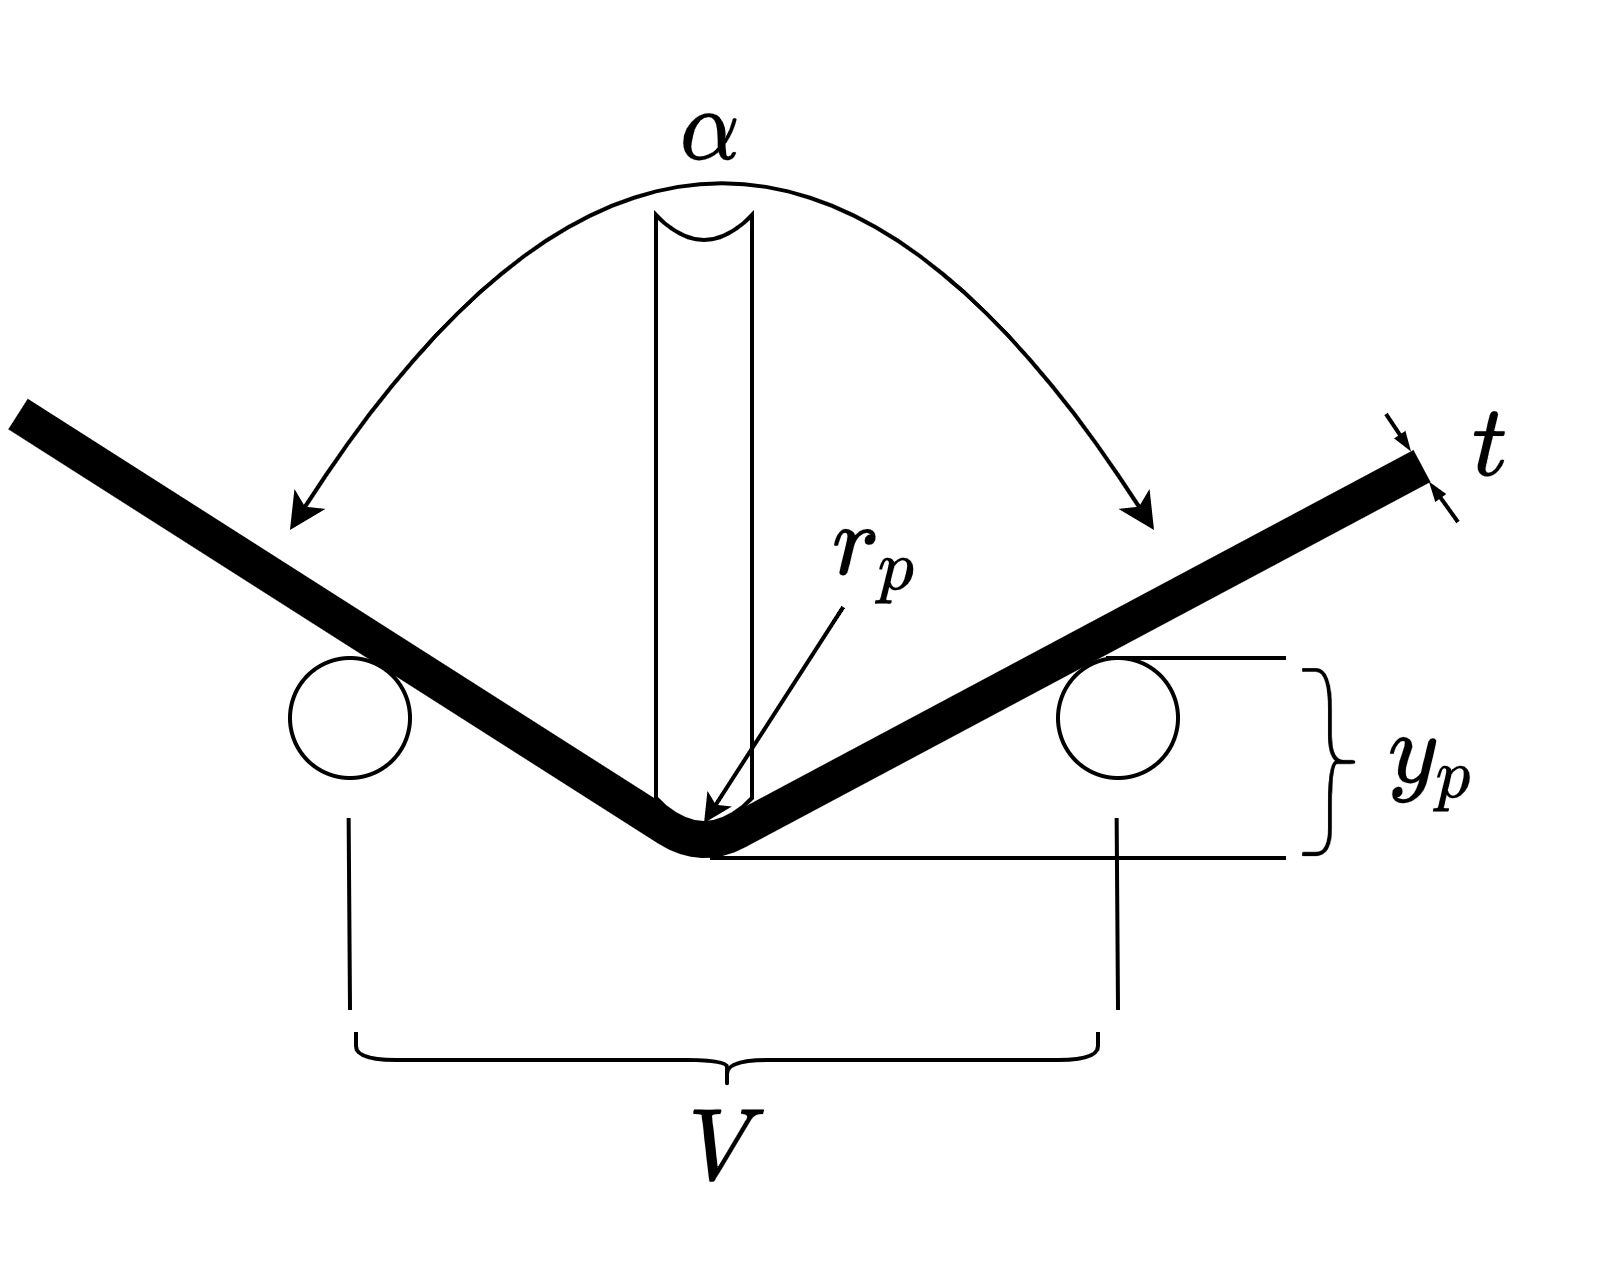
\includegraphics[trim=left botm right top, width=0.6\textwidth,
            clip]{chap4/images/process_parameters}
    \end{tcolorbox}
    \caption{\textbf{Process parameters:} Sheet bending angle ($\alpha$), sheet
    thickness ($t$), punch
    penetration ($y_p$), die opening ($V$) and punch radius ($r_p$)}
    \label{fig:process_parameters}
\end{figure}

To ensure consistent results, a set of constant and variable parameters were selected.
The punch was never changed and therefore the punch radius ($r_p$) is a constant parameter.
Also the length and the width of the used metal sheets were standardized to 20 mm and 80 mm, respectively.

The hold time, which refers to the duration that the punch remains stationary
after reaching the maximum displacement ($y_p_{\max}$), was set to a minimum of 1 second.
The punch force threshold was set to 1 N, meaning that the punch was initially moved at
a higher speed until the force reached 1 N, and then moved at a slower speed of 80 mm
/min until the $y_p_{\max}$ was reached.

\begin{table}[htb]
    \begin{tcolorbox}[arc=0pt,boxrule=0.5pt]
        \sisetup{group-minimum-digits = 4}
        \centering
        \begin{tabular}{lll}
            \toprule
            \thead{\textbf{Parameter}} & \thead{\textbf{Values}} &
            \thead{\textbf{Unit}}
            \\
            \midrule
            Punch radius & 5 & $mm$
            \\
            \hdashline
            Sheet width & 20 & $mm$
            \\
            \hdashline
            Sheet length & 100 & $mm$
            \\
            \hdashline
            Punch speed & 80 &
            $mm/min$ \\
            \hdashline
            Punch speed up (after bend) & 8 &
            $mm/min$ \\
            \hdashline
            Hold time & 1 & $s$ \\
            \hdashline
            Punch force threshold & 1 & $N$
            \\
            \bottomrule
        \end{tabular}
    \end{tcolorbox}
    \label{tab:experimental-setup-constant-parameters}
    \caption{Constant parameters in th eperimental setup}
\end{table}

The experiment involved varying three parameters: The die opening ($V$), the
punch penetration ($y_p$), and the thickness of the metal sheet ($t$).
The die opneing was varies from 10 mm to 50 mm, the maximum punch penetration was varied from 2.5 mm to 20 mm and the
metal sheet was varied from 0.5 mm to 2 mm.
These parameters and their values are displayed in
\cref{tab:experimental-setup-variable-parameters}.

\begin{table}[h]
    \begin{tcolorbox}[arc=0pt,boxrule=0.5pt]
        \sisetup{group-minimum-digits = 4}
        \centering
        \begin{tabular}{lll}
            \toprule
            \thead{\textbf{Parameter}} & \thead{\textbf{Values}} &
            \thead{\textbf{Unit}}
            \\
            \midrule
            %  \unit{(Kcal\per\mole)\squared}}} & \thead{RMSD l.b.} &
            %  \thead{RMSD u.b.}  \\
            \midrule
            Punch penetration  $y_p$ & 2.5, 5, 7.5, 10, 12.5, 15, 17.5, 20 &
            $mm$ \\
            \hdashline
            Die opening        $V$ & 10, 20, 30, 40, 50
            & $mm$ \\
            \hdashline
            Thickness          $t$ & 0,5, 1, 1.5, 2, 2.5, 3
            & $mm$ \\
            \bottomrule
        \end{tabular}
    \end{tcolorbox}
    \caption{Varying parameters in the experimental setup}
    \label{tab:experimental-setup-variable-parameters}
\end{table}

\subsection{Measuring The Spring Back} \label{subsec:measuring_the_spring_back}
The output data included various data points that were used to calculate the spring back.
Key parameters for this calculation were the force, punch travel, and time
which are illustrated in \cref{fig:springback_measured}.
The blue line is representing the for force while the gray line is representing the punch travel.
The punch movement is measured as soon as the displacement sensor is activated with when it notices a difference of 1 N
which is the case when the punch touches the metal sheet.

% TODO stimmt das?
It can be seen that before the punch touches the metal sheet there is already a force measured of about 10 N, this is
the case because the punch is moving at a speed of 80 mm/min which is relatively fast and so the displacement sensor
is activated before the punch touches the metal sheet.
The wait time at of 1 second $y_p_{max}$ is a limitation of the machine and can not be
changed and therefore is always a part of the experimental setup.

At the point where the punch is moved fully down, known as $y_p_{max}$, there is a noticeable decrease in force, as
observed in \cref{fig:springback_measured}. This phenomenon is most likely attributed to the released friction (
personal communication with Prof. Dr.-Ing. Marco Schneider).

\begin{figure}[H]
    \begin{tcolorbox}[arc=0pt,boxrule=0.5pt]
        \centering
        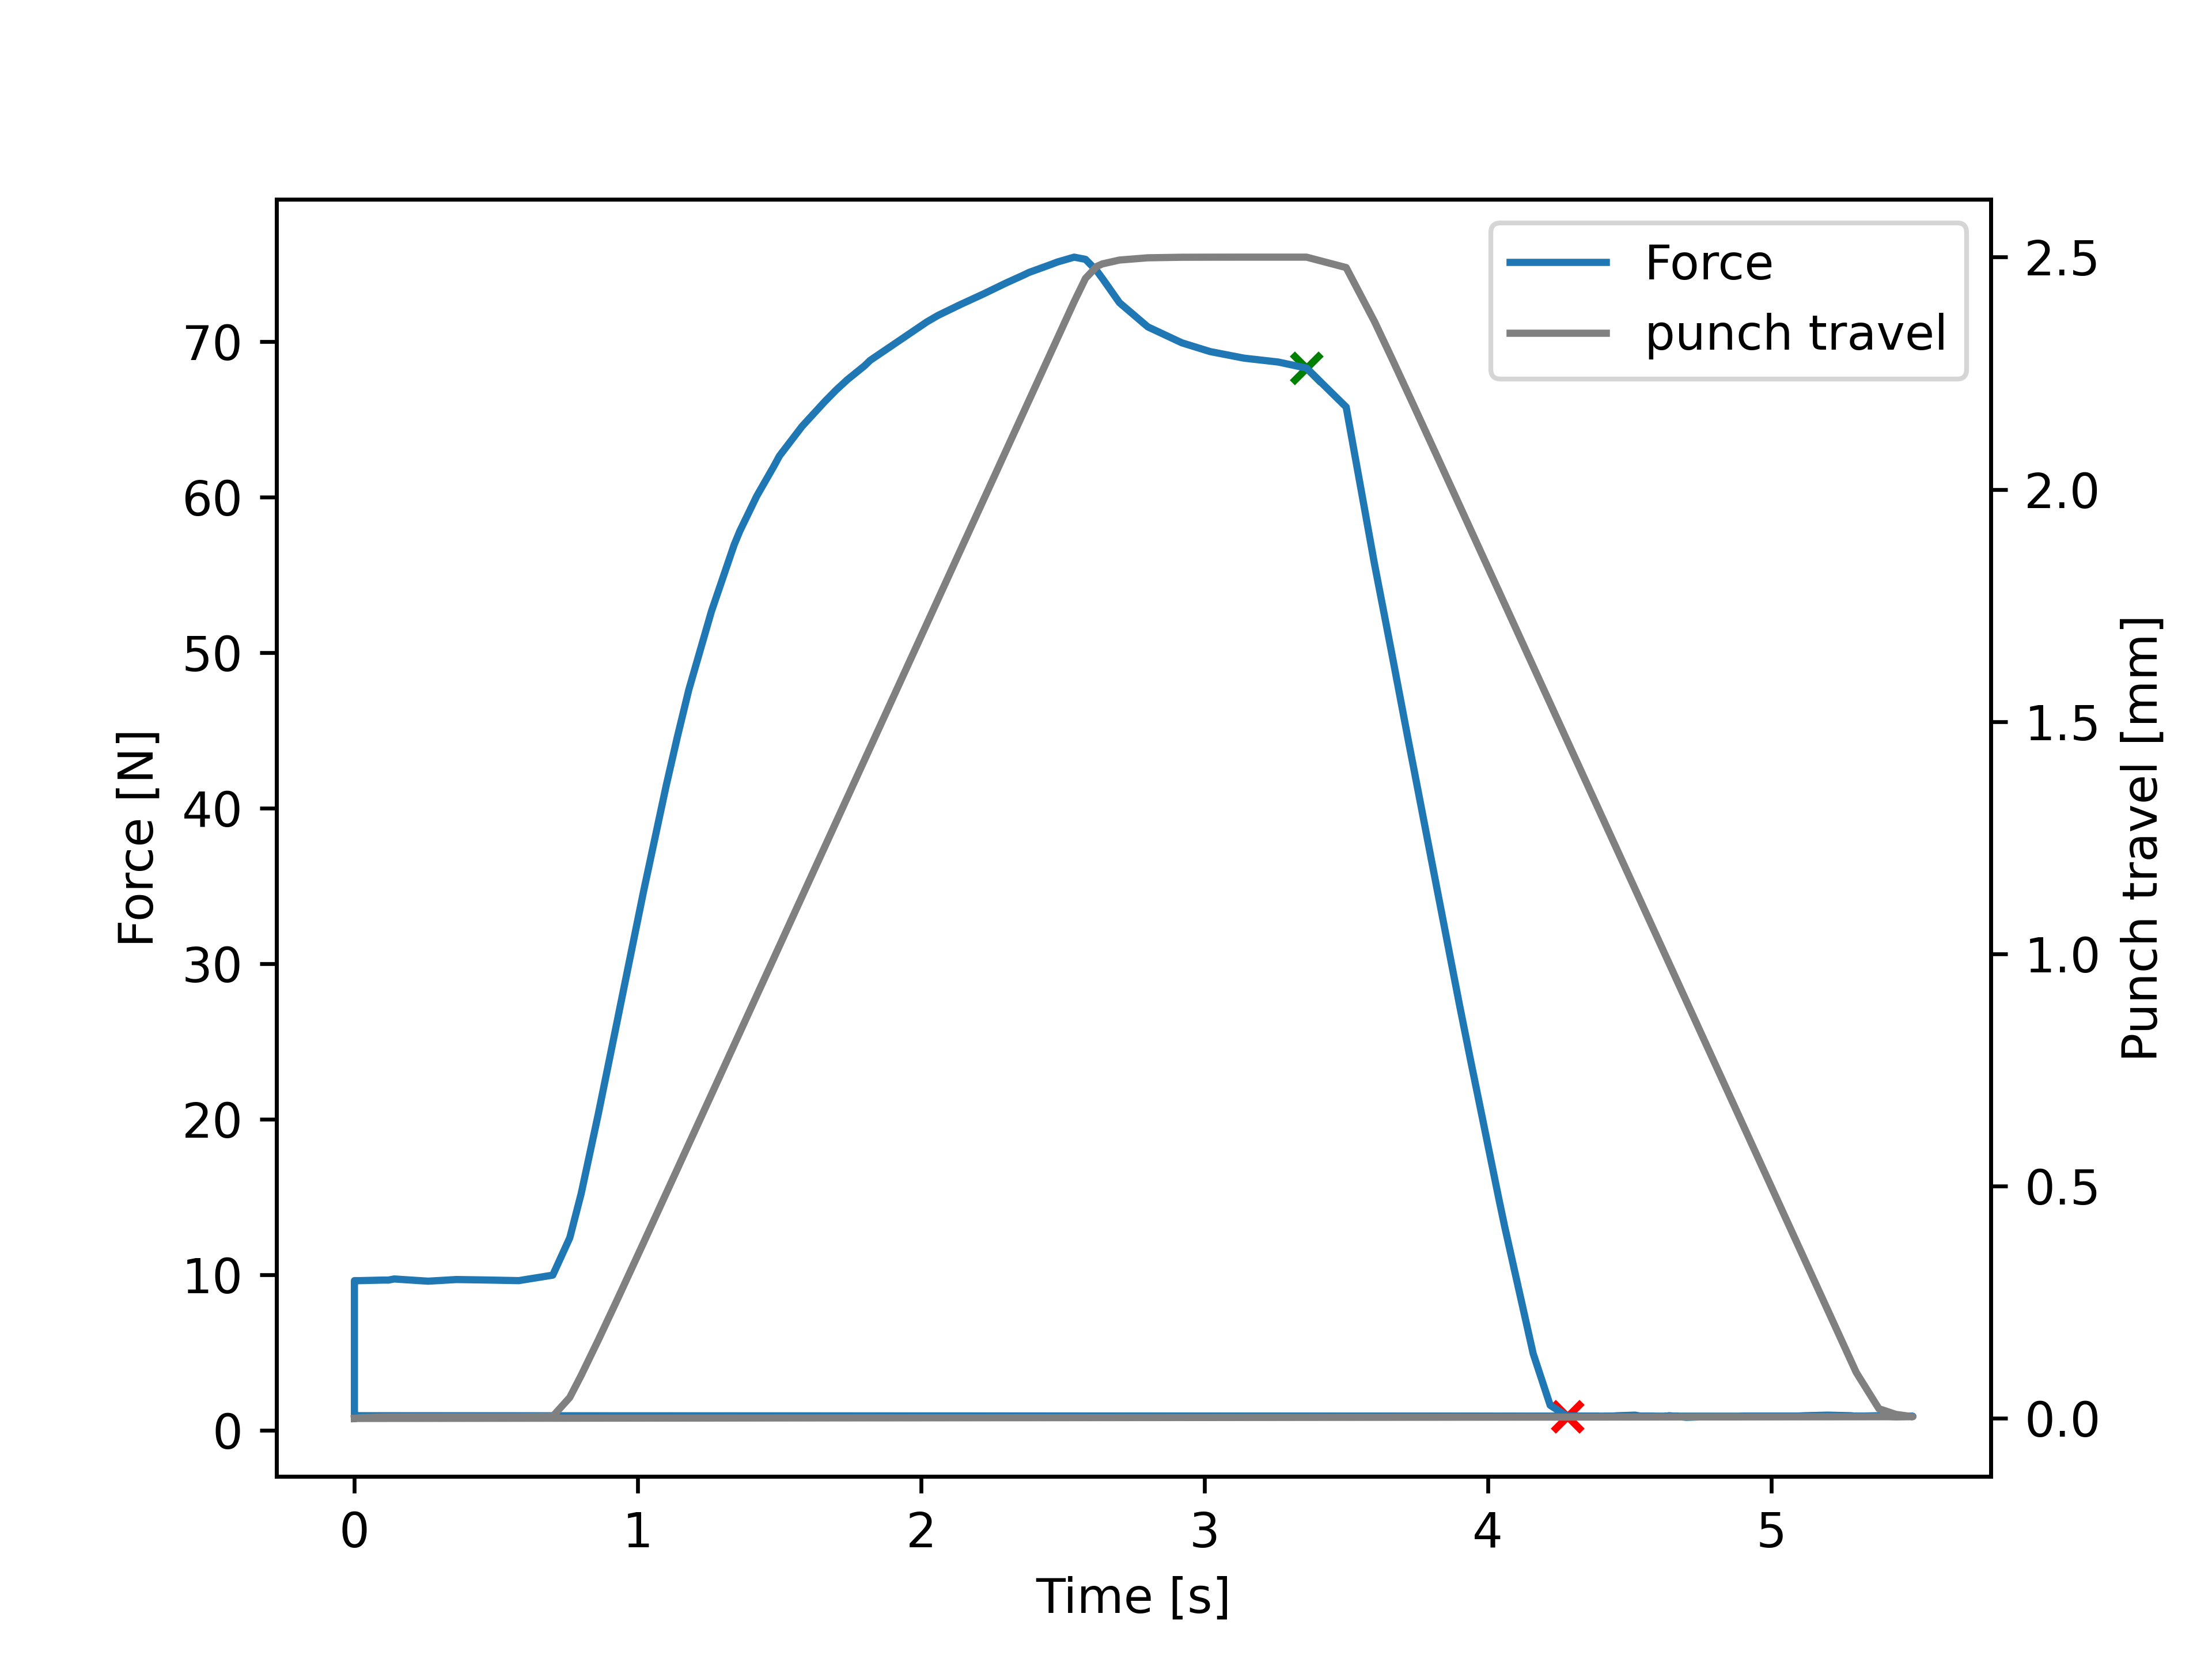
\includegraphics[width=0.7\textwidth]{chap4/images/springback_measured}
    \end{tcolorbox}
    \caption{\textbf{Spring back measured:} A steel metal sheet was bent with a punch penetration of 5
    mm the spring back is 0 .37 mm. The blue line shows the force and the blue line shows the punch penetration.
    The distance between the green and the red point repesents the spring back distance.}
    \label{fig:springback_measured}
\end{figure}

\subsection{Dataset Exploration}\label{subsec:dataset-exploration}
The dataset was explored using the \textit{pandas}~\cite{mckinney-proc-scipy-2010}
and the \textit{matplotlib}~\cite{Hunter:2007} python library.
The goal of this section is to give the reader an overview of the dataset and
to show the relationship between the features and the dependent variable.

\subsubsection{Features}
The output data of the bending machine consisted of 26 features, which are listed in
the appendix.
Only three features - force, distance $y_p$, and time - are relevant for
calculating the spring back, as described in the previous section~\ref{subsec:measuring_the_spring_back}.
These three features were combined with the calculated spring back to form the final
dataset, which contained a total of 404 data points generated.
An example of the dataset is presented in \cref{tab:dataset_example}.

\begin{table}[h]
    \begin{tcolorbox}[arc=0pt,boxrule=0.5pt]
        \sisetup{group-minimum-digits = 4}
        \centering
        \begin{tabular}{l|llll}
            \toprule
            \thead{\textbf{index}} & \thead{\textbf{Punch Penetration}} &
            \thead{\textbf{Spring Back}}
            &
            \thead{\textbf{Thickness}}
            & \thead{\textbf{Die Opening}}
            \\
            1   & 5.0  & 0.6667 & 2.0 & 50  \\
            \hdashline
            2   & 15.0 & 0.9164 & 2.0 & 50  \\
            \hdashline
            3   & 10.0 & 0.6829 & 2.0 & 50  \\
            \hdashline
            ... & ...  & ...    & ... & ... \\
            \hdashline
            396 & 5.0  & 0.6667 & 3.0 & 10  \\
            \bottomrule
        \end{tabular}
    \end{tcolorbox}
    \caption{Excerpt from the dataset with 404 data points used in this study.}
    \label{tab:dataset_example}
\end{table}

\cref{fig:v30_springbacks} depicts the spring backs that were observed in a specific
subset of the data where the die opening is 30 mm.
The horizontal axis, labeled as the x-axis, represents the punch penetration distance, while the vertical axis,
labeled as the y-axis, represents the spring back.
In order to clearly illustrate all the data points, the mean of the spring backs has been plotted as a line.

Upon examining the figure, two general trends become evident.
Firstly, a lower thickness of the metal sheet leads to a higher degree of spring back.
Secondly, a higher punch penetration distance leads to a higher spring back as well.
It is also apparent that there is a non-linear relationship between the punch penetration and the spring back.
These trends are also observed for other die openings and therefore apply for the whole dataset.

\begin{figure}[h]
    \begin{tcolorbox}[arc=0pt,boxrule=0.5pt]
        \centering
        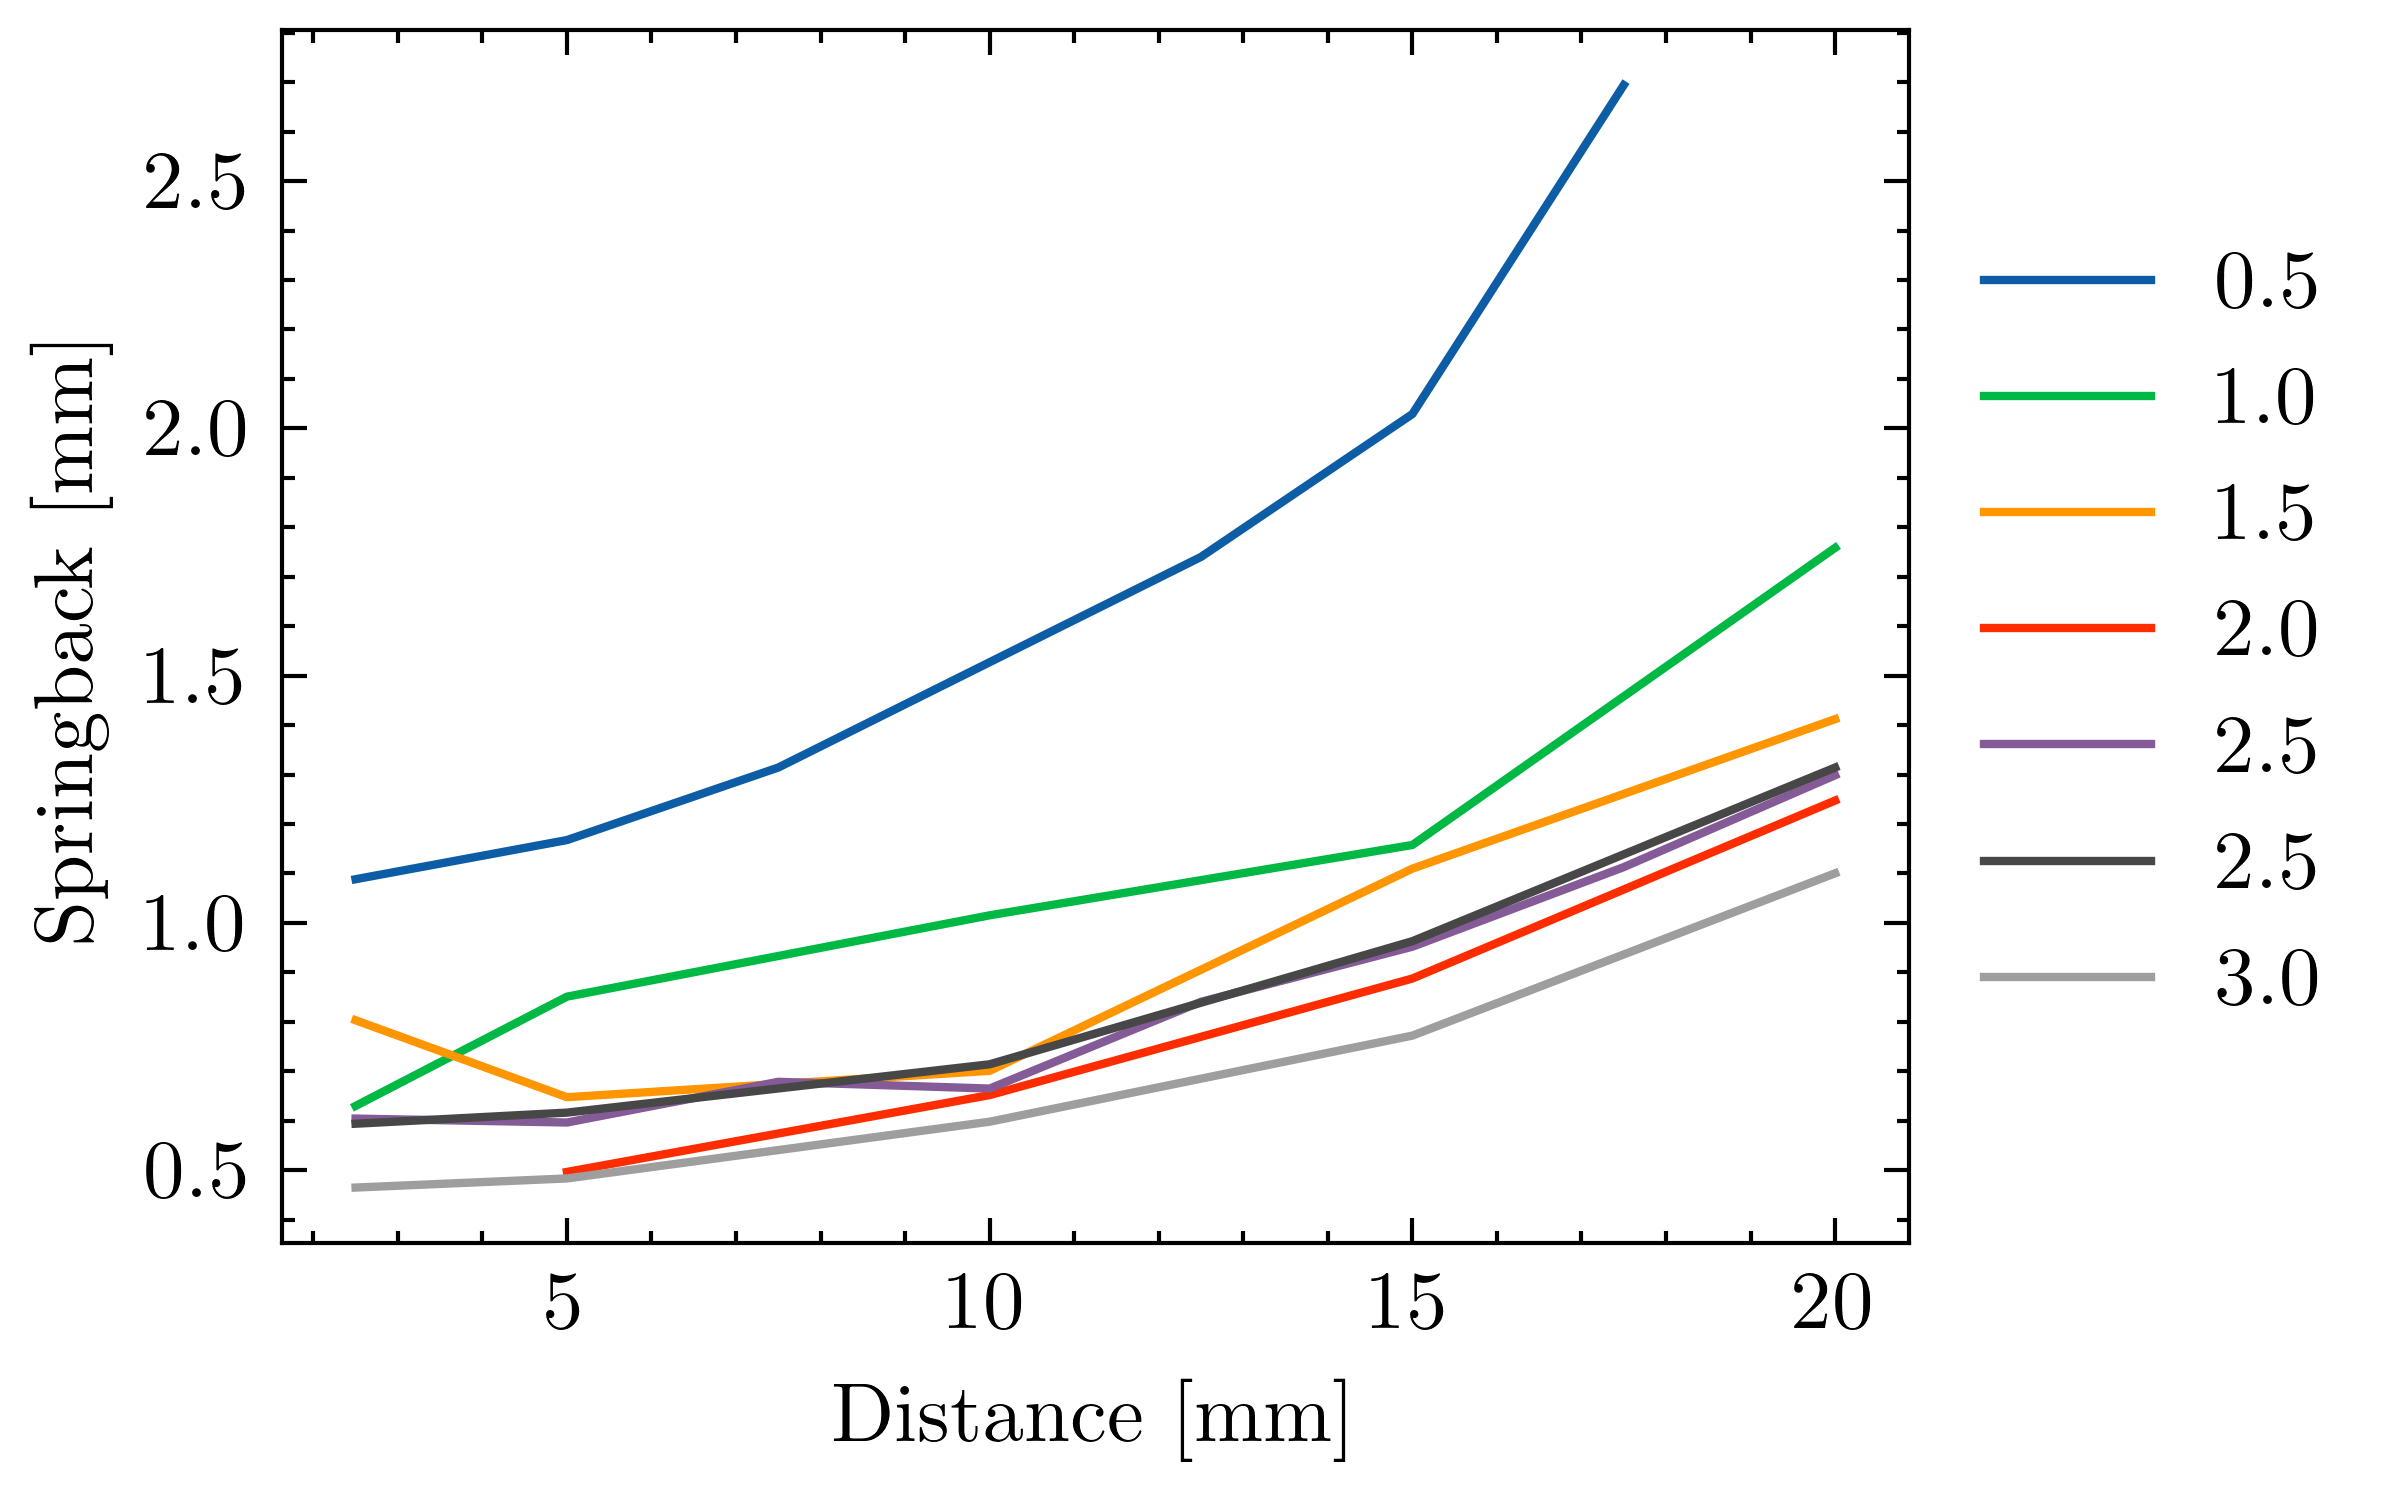
\includegraphics[width=0.8\textwidth]{chap4/images/all-springbacks-consolidated}
    \end{tcolorbox}
    \caption{All measured springbacks for the die opening $V30$ are shown. }
    \label{fig:v30_springbacks}
\end{figure}

\subsubsection{Data Quality}
The dataset was carefully created in a controlled experimental environment to ensure precise and accurate
measurements of the samples.
As a result, the dataset exhibits a minimal number of outliers and high data quality,
which is a crucial prerequisite for developing reliable machine learning models.

\cref{fig:train_test_split} illustrates that the dataset encompasses nearly all possible combinations of the
process parameters, namely $V$, $t$, and $y_p$.
The $y_p$ values in the dataset are uniformly distributed and consistently ranged between 2.5 and 20 mm.
Furthermore, the dataset was continuously expanded with new data points throughout the project to enhance its size and
diversity.
The figure also show the test-train split which will be explained in \cref{fig:train_test_split}.

\begin{figure}[h]
    \begin{tcolorbox}[arc=0pt,boxrule=0.5pt]
        \centering
        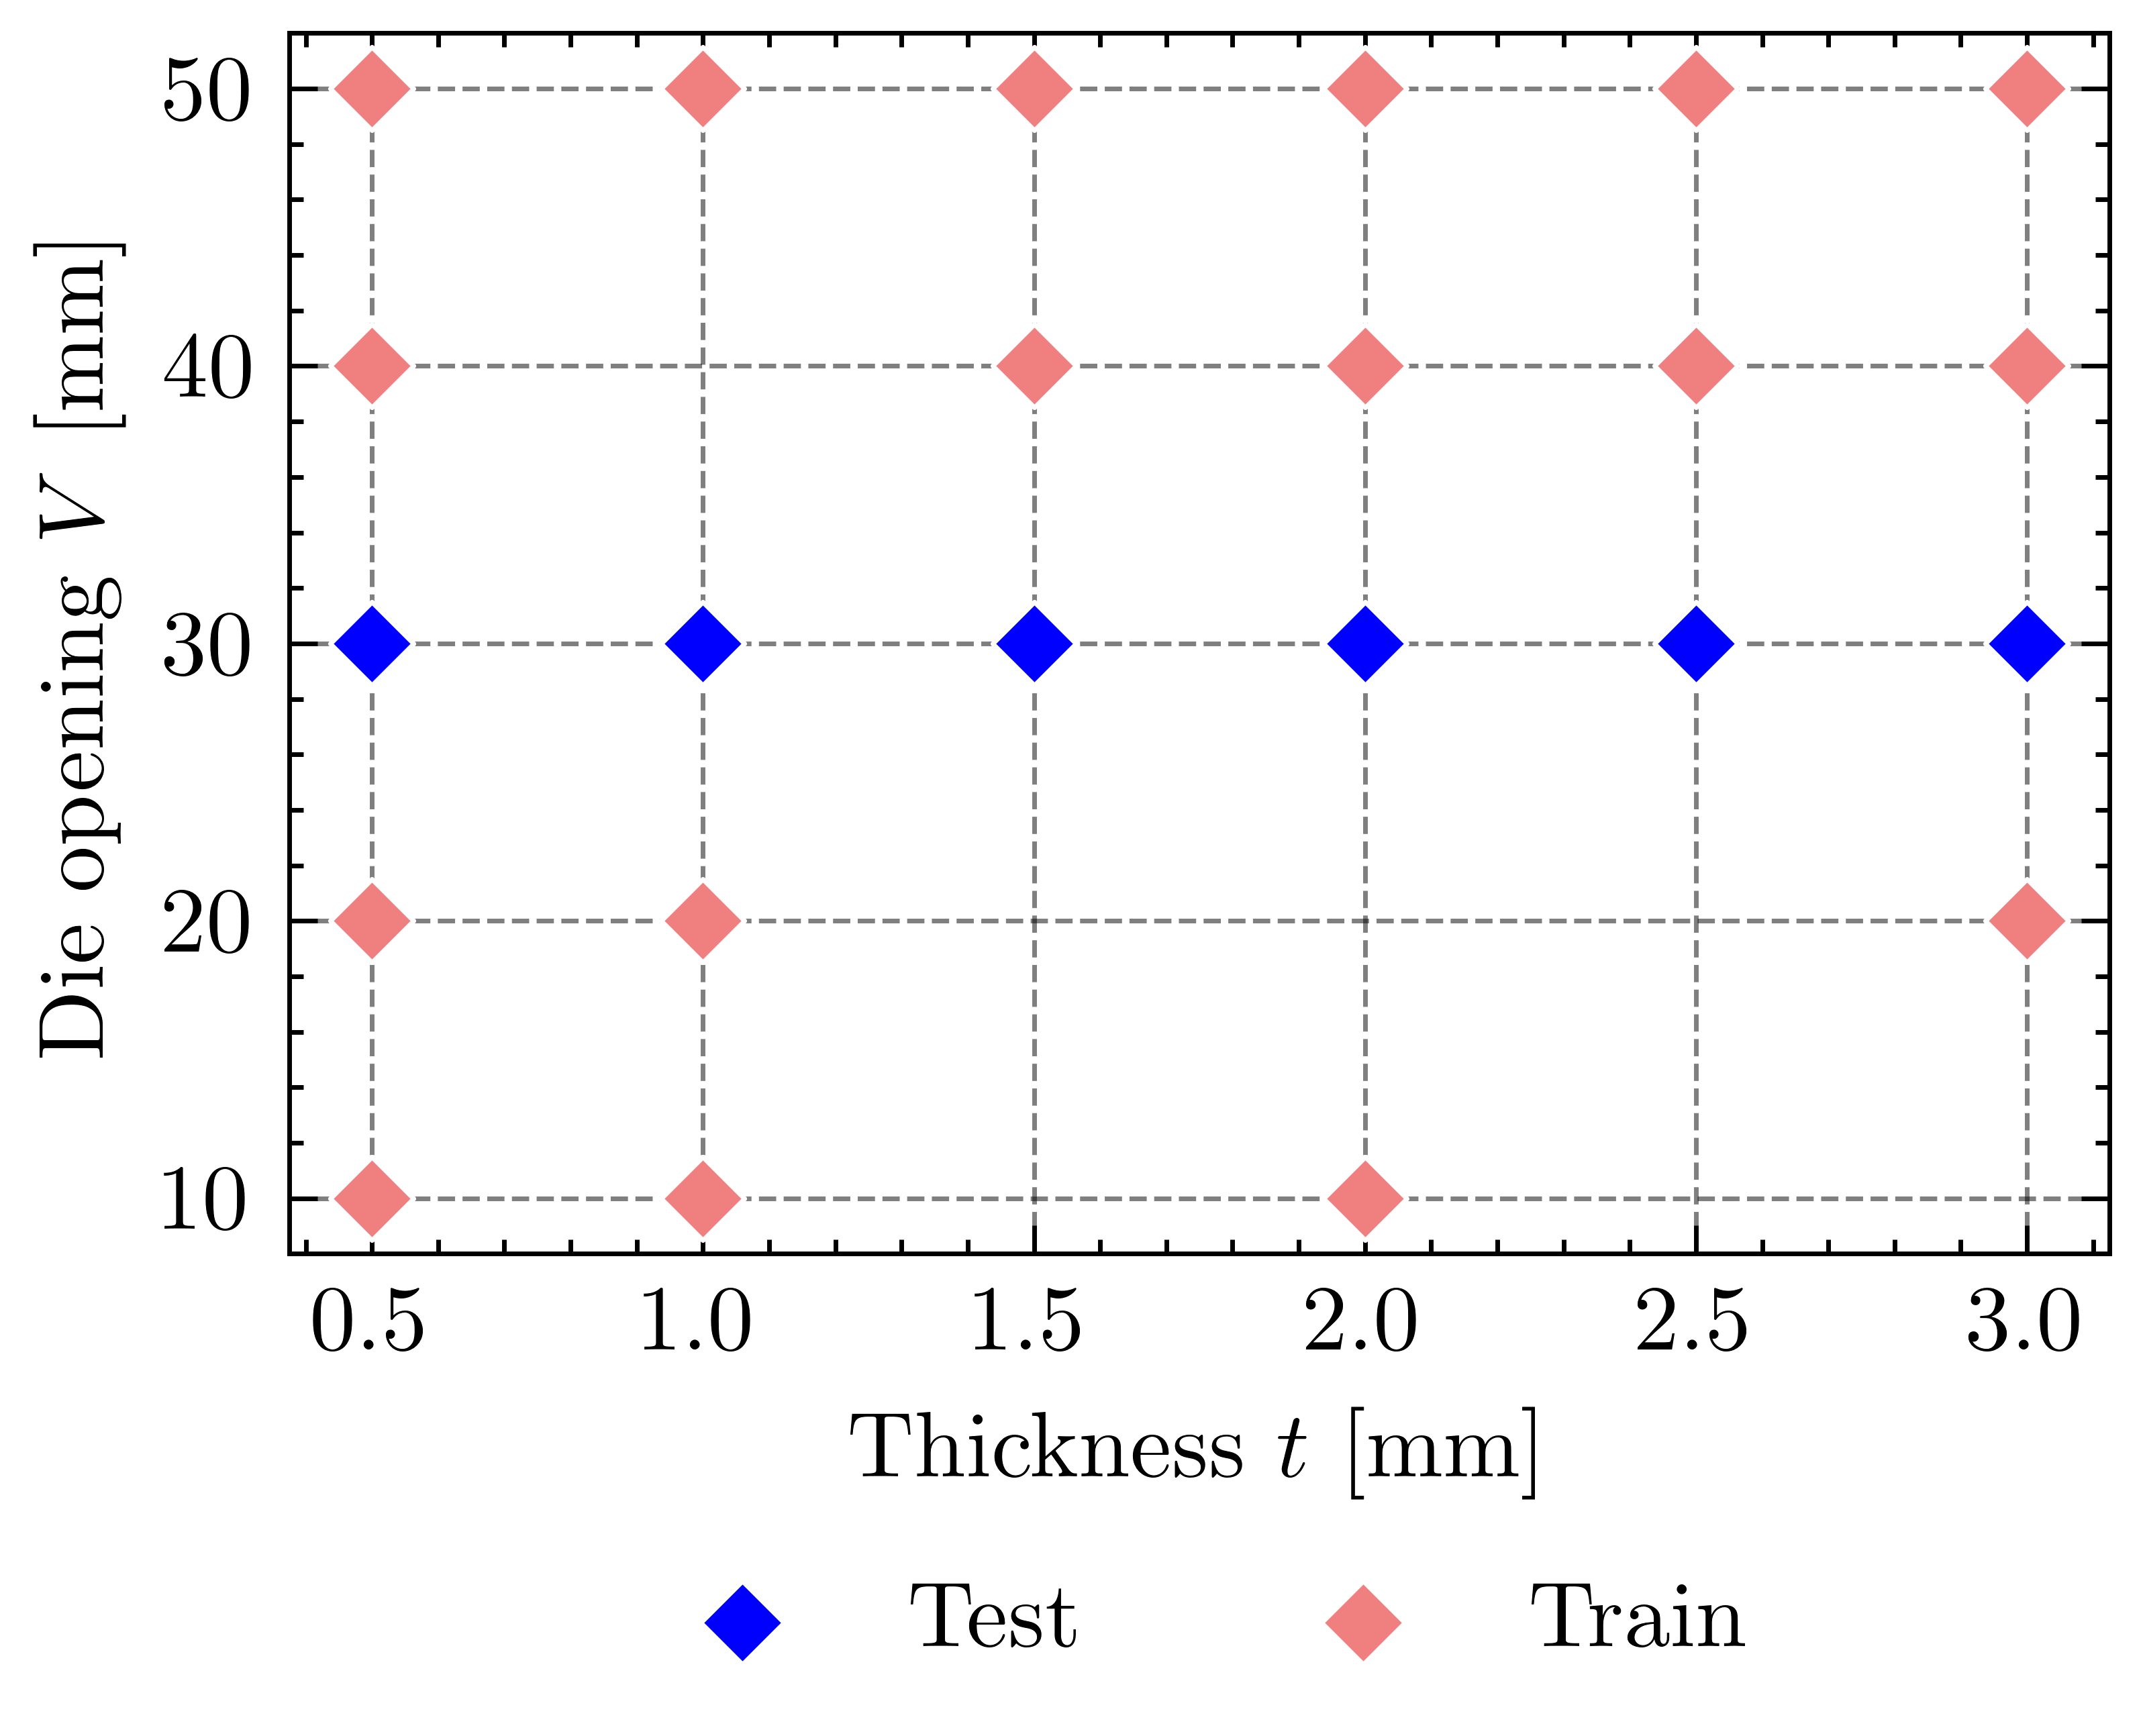
\includegraphics[width=0.8\textwidth]{chap4/images/test_train_split}
    \end{tcolorbox}
    \caption{The training and test dataset.}
    \label{fig:train_test_split}
\end{figure}

The following gaps can be seen in the dataset: Metal sheet thickness with $V10$  after 1 mm could not be measured
because the die opening was too small to fit the metal sheet.
Also data for $V$ 20 and $t$ 2,5 as well as $V$ 40 and $t$ 1 are missing, for time related reasons.

Throughout the data collection and expansion process, any outliers and incorrect measurements were identified and
removed from the dataset to maintain its high quality.
%However, it is worth noting that the data may not fully reflect real-world scenarios where various factors, such as
%measurements errors, noise and bias can impact data quality.
%In later sections, data quality issues will be intentionally introduced to evaluate the models' robustness to such
%challenges.
This will provide insights into how well the machine learning models perform in more realistic scenarios and aid in
developing more effective models for practical applications.

\subsection{Data Preprocessing}\label{subsec:data-preprocessing}
To normalize the independent features $y_p$, $V$, and $t$, as well as the dependent feature $spring\_back$, the
\texttt{MinMaxScaler} or, in some cases, the \texttt{StandardScaler} from the
\texttt{scikit-learn}~\cite{scikit -learn} library where employed.

The \texttt{MinMaxScaler} scales the data between 0 and 1 and the scaler was fit on the training data and
subsequently used to transform the test data.
It is important to note that scaling was only performed on the training data, as cross-validation was later employed
to tune and evaluate the models.
Scaling the entire dataset before the split could result in data leakage, as the minimum and maximum values of the
test data would be used to scale the training data.

The data split is depicted in \cref{fig:train_test_split}.

\subsection{Computational Setup}\label{subsec:computational-setup}
A ThinkPad X1 Carbon 2019 with an Intel Core i7-10610U CPU @ 1.80GHz and 16 GB RAM was utilized to train the machine
learning models.
The OS used was Ubuntu 20.04.2 LTS on which the code was written in Python 3.8.5 with the PyCharm IDE.
The code can be found on GitHub and on the the CD accompanying this thesis.
The libraries used are listed in \cref{tab:libraries}.

\captionsetup{width=1\textwidth}
\begin{table}[h]
    \begin{tcolorbox}[arc=0pt,boxrule=0.5pt]
        \sisetup{group-minimum-digits = 4}
        \centering
        \begin{tabular}{llll}
            \toprule
            \thead{\textbf{Library}} & \thead{\textbf{Version}} & \thead{\textbf{Author}} \thead{\textbf{Use}}
            &
            \\
            \toprule
            Sci-Kit Learn & 1.2.2 & ~\cite{scikit-learn} \\
            \hdashline
            numpy~ & 1.23.2 & ~\cite{harris2020array} \\
            \hdashline
            pandas & 1.5.1 & ~\cite{mckinney-proc-scipy-2010} \\
            \hdashline
            matplotlib & 3.6.2 & ~\cite{Hunter:2007} \\
            \hdashline
            scienceplots & 2.0.1 & ~\cite{SciencePlots} \\
            \hdashline
            seaborn & 0.12.2 & ~\cite{Waskom2021} \\
            \bottomrule
        \end{tabular}
    \end{tcolorbox}
    \caption{Libraries used for the machine learning models.}
    \label{tab:libraries}
\end{table}

A note to the citations of the libraries.
All of the above libraries are well documented on their website.
Libraries used for the machine learning models.

Upon examining the correlation matrix depicted in \cref{fig:correlation_matrix}, the correlation is between 0 and 1,
the higher the value the stronger the correlation.
It is evident that the distance and spring back features exhibit a stronger correlation
than the other features.
This correlation is to be expected since punch penetration $y_p$ is the primary factor
that influences the amount of spring back.
The other features are not connected with each other, demonstrating the lack of multicollinearity, which is a
desirable trait for machine learning models.

The correlation matrix was generated using the \texttt{heatmap} function from the \textit{seaborn} library
~\cite{Waskom2021}.

\begin{figure}[H]
    \begin{tcolorbox}[arc=0pt,boxrule=0.5pt]
        \centering
        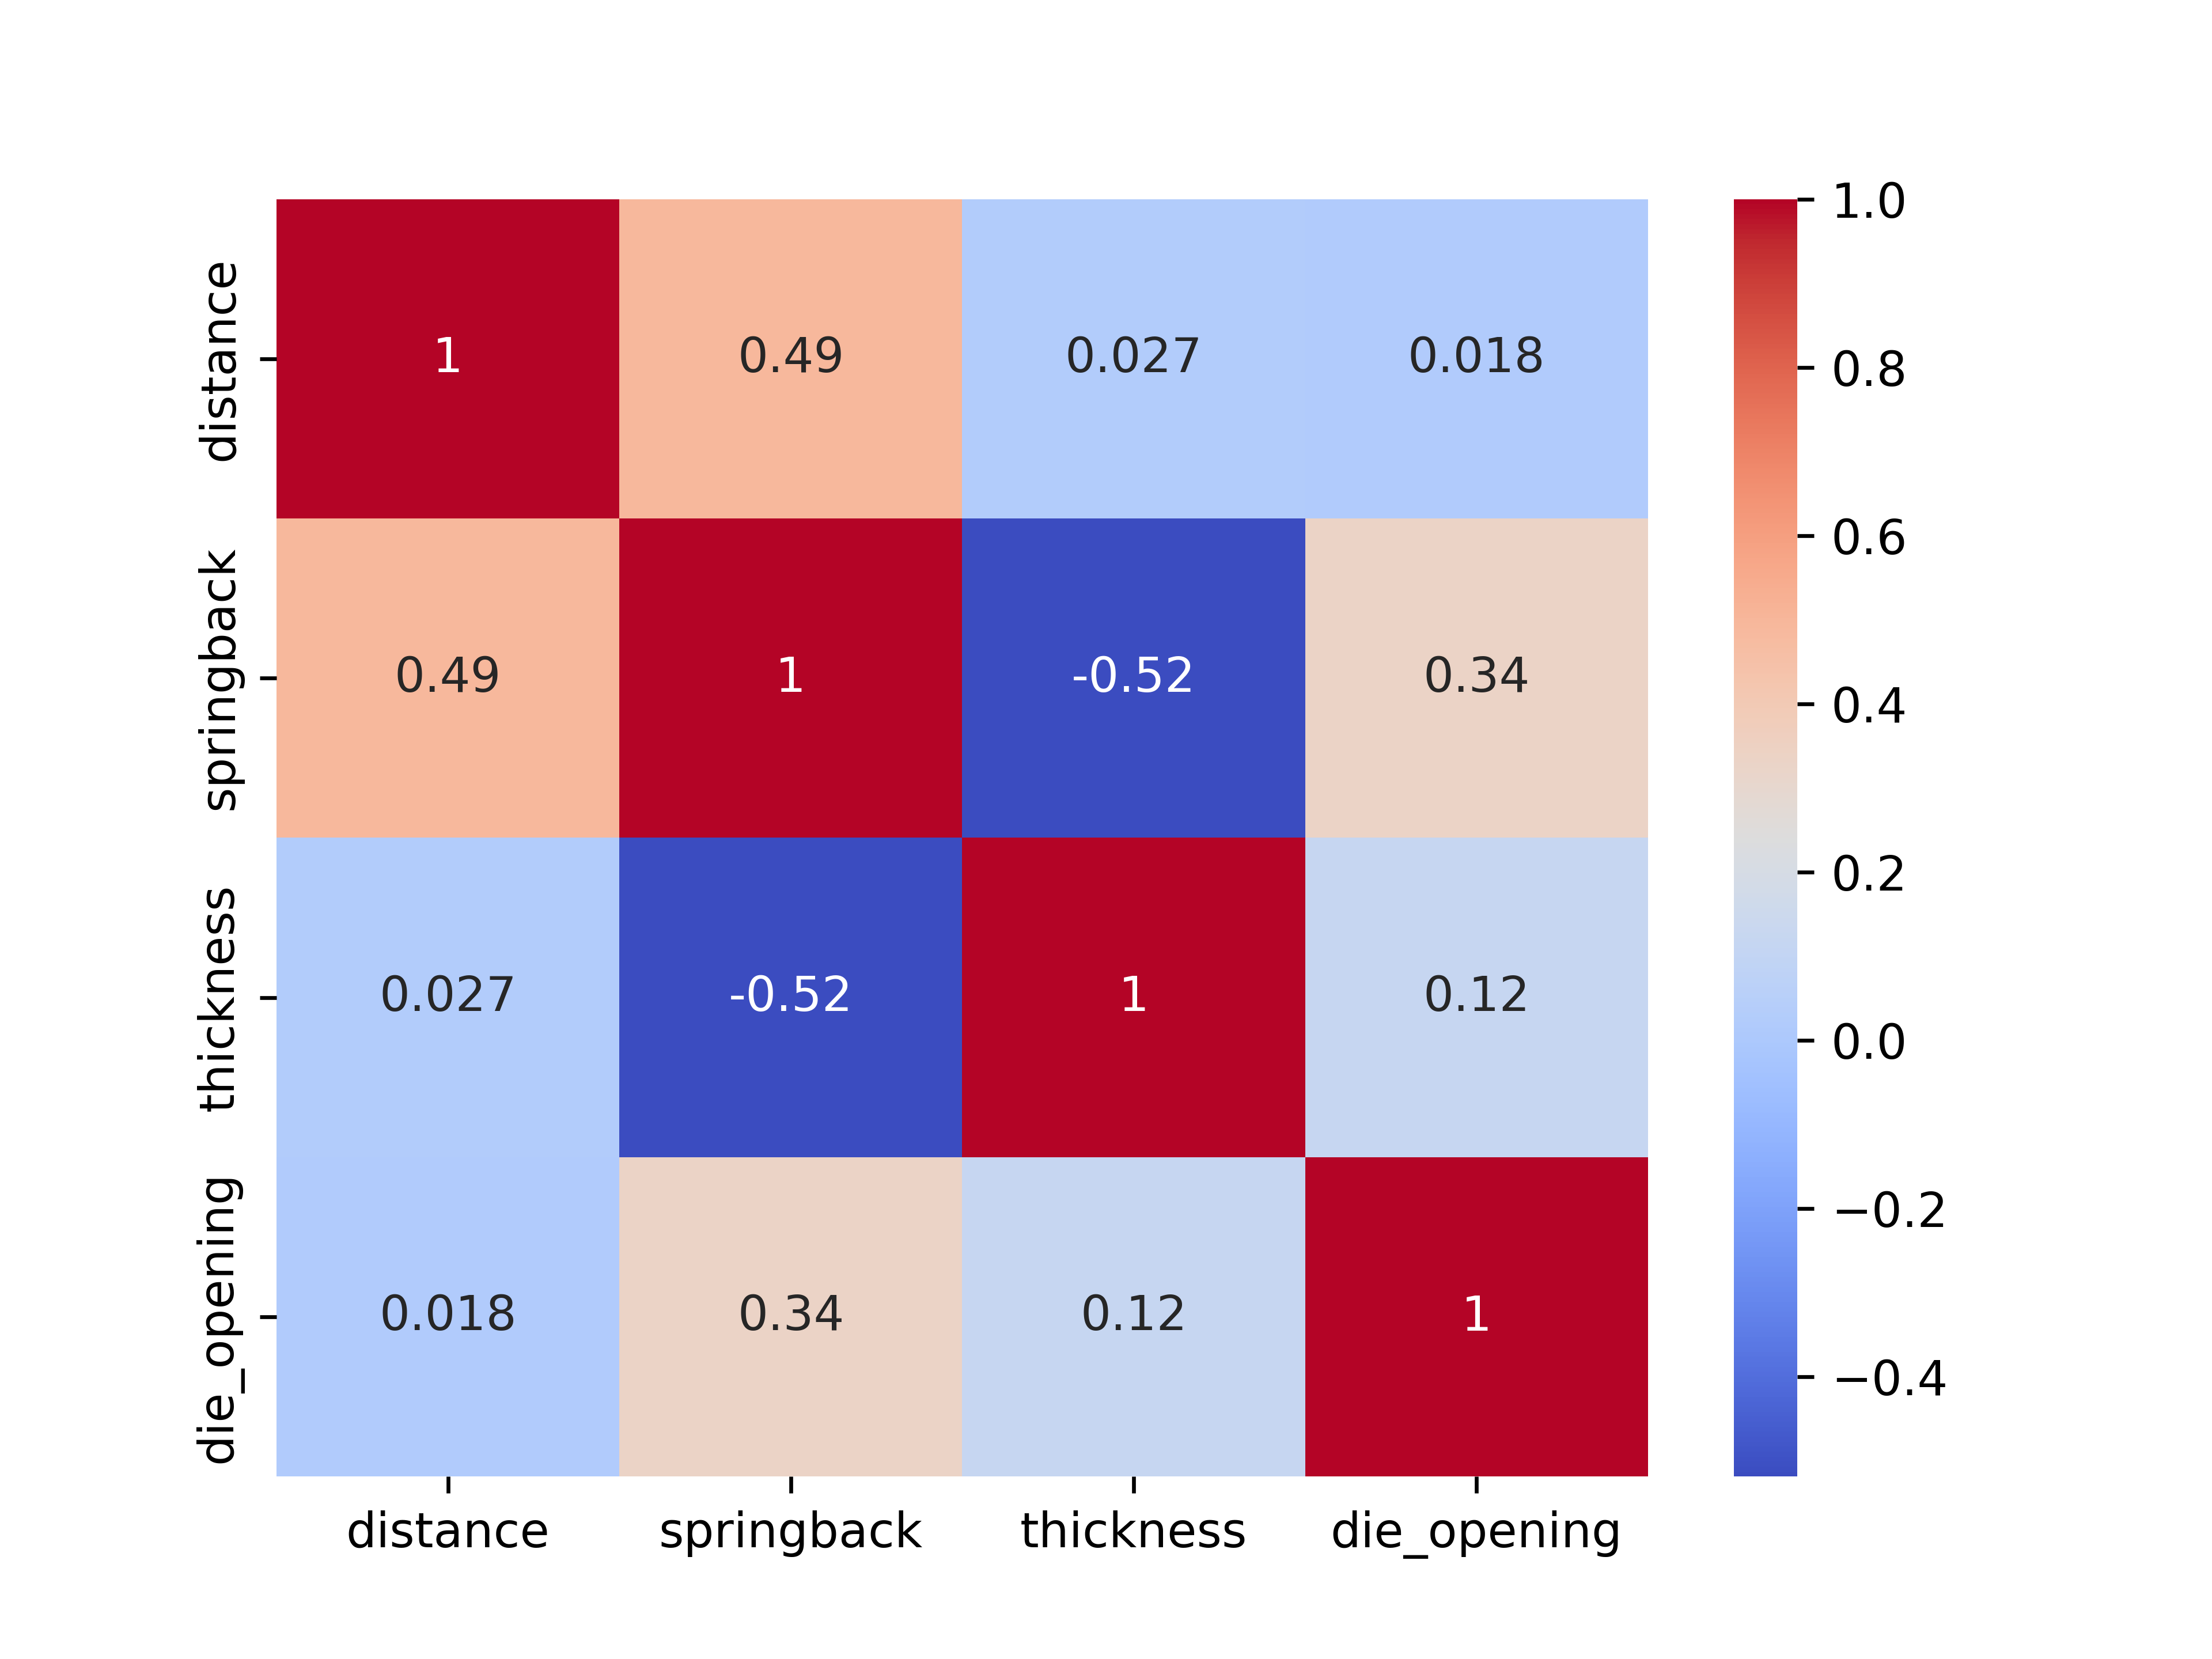
\includegraphics[width=0.7\textwidth]{chap4/images/correlation_matrix}
    \end{tcolorbox}
    \caption{Correlation matrix generated with a Random Forest Regressor model}
    \label{fig:correlation_matrix}
\end{figure}


\section{Model Selection}\label{sec:model-selection}
This thesis focuses on the utilization of Supervised Machine Learning models to predict
spring back.
Therefore, a selection of the most common machine learning models where used, based on
the systematic literature review of
~\cite{dridi2021supervised}.
\cite{dridi2021supervised} defines eight widely used supervised machine learning models in the paper.
These models are Logistic Regression, Support Vector Machines, Decision Trees, Random Forests, AdaBoost, Naive Bayes
, and K-Nearest Neighbors.

However, Naive Bayes and K-Nearest Neighbors are not used in this thesis since they are typically
utilized for classification problems.
Furthermore, in order to compare the performance of the other models, a Linear Regression model
and a Multi-Layer-Perceptron were also employed.
The models can be classified into five categories: Logic-based learning, instance-based learning, Deep learning, and
Support Vector Machines~\cite[p. 8]{dridi2021supervised}.

\subsection{The Baseline Model}\label{subsec:regression-models}
In this study, a Linear Regression (LR) model is employed as the baseline model.
Linear regression a widely used method to predict a continuous output (dependent variables) based on a set
of input features (independent variables).
The goal of a \ac{LR} model is to find the best-fitting straight to explain the relationship between the dependent
(spring back) and independent (die opening, thicnkess, punch penetration)
variables
~\cite[pp. 45--46]{muller_introductionmachinelearning_2016}.
This so called regression line can be express as shown in \xref{eq:linear-regression}, which is taken from
Müller and Guido (2016)
~\cite[p. 45]{muller_introductionmachinelearning_2016}.

\begin{tcolorbox}[arc=0pt,boxrule=0.5pt]
    \begin{equation}
        \hat{y} = w[0] * x[0] + w[1] * x[1] + ... + w[p] * x[p] + b
        \label{eq:linear-regression}
    \end{equation}
\end{tcolorbox}

The linear regression model is trained by minimizing the sum of squared errors between predicted and actual values.
The values $x[0]$ to $x[p]$ indicate the properties of a single data instance, with $p$ being the number of
features.
The learned parameters of the model are $w$ and $b$, and $\hat{y}$  is the prediction generated by the model.

The Mean Squared Error is calculated by adding together the squared discrepancies between the predicted and true
values~\cite[p. 47--68]{muller_introductionmachinelearning_2016}.
This model presumes a linear relationship between the independent and dependent variables.
The dataset exploration in \cref{subsec:dataset-exploration}, on the other hand, revealed a nonlinear relationship
, implying that the linear regression model may not deliver reliable predictions.
Despite this disadvantage, the model can be used as a baseline against which other models can be compared.

%% TODO hier ist noch Molnar
%Another reason to use linear regression is its interpretability and simplicity.
%The linear relationship between inputs and targets makes model interpretation
%straightforward
%~\cite[p. 37]{molnar2020interpretable}.

%Another reason why an \ac{LR} model is used in this study is its interpretability and simplicity.
%The linearity of the relationship between the inputs and the target makes the
%interpretation of the model straightforward
%~\cite[p. 37]{molnar2020interpretable}.

\subsection{Support Vector Regression (SVR)}\label{subsec:support-vector-regression-(svr)}
Support Vector Machines (SVMs) are a popular approach for solving classification problems.
To understand how the SVM algorithm works, it can be helpful to approach the problem from a geometric perspective.
For example, a two-dimensional space as shown in \cref{fig:svm-example} can be considered, where each data point
has a class assigned, in this case, either red or blue.
The SVM algorithm seeks to identify a line (hyperplane) that separates the data points into different classes in the
best way possible which means that there is the largest possible distance between the line and the
nearest points of each class
~\cite[pp. 92--96]{muller_introductionmachinelearning_2016}.

The points that lie closest to the hyperplane are called support vectors, these define the margin which is tried to be
maximized by the algorithm and therefore are important for determining the optimal position of the hyperplane
~\cite[p. 42]{awad_efficientlearningmachines_2015}.
The hyperplane serves as a decision boundary that separates the data points into different
classes~\cite[p. 11]{awad_efficientlearningmachines_2015}
, in the example the points on the one side of the hyperplane are classified with the blue class while the
points on the other side are classified with the red class

Since each feature in the dataset is formulated as one dimension in the geometrical space, visualizing the hyperplane
is usually not as straightforward as in the example depicted in Figure~\ref{fig:svm-example}.
In the case of the spring back dataset, for instance, the hyperplane would be a three-dimensional plane, but it is
not uncommon to have spaces with even higher dimensions.
The algorithm seeks a hyperplane in an N-dimensional space (where N is the number of features) in order to
effectively separate and classify data points
~\cite[]{awad_efficientlearningmachines_2015}.

\begin{figure}[H]
    \begin{tcolorbox}[arc=0pt,boxrule=0.5pt]
        \centering
        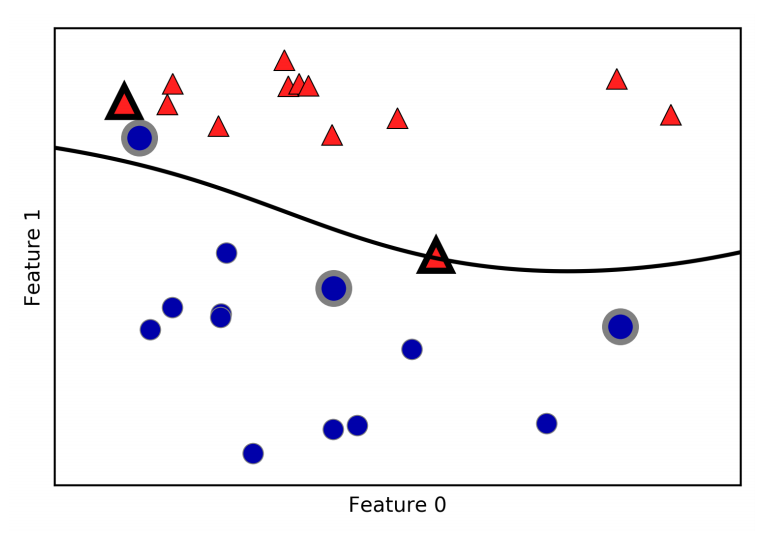
\includegraphics[width=0.7\textwidth]{chap4/images/svm_example}
    \end{tcolorbox}
    \caption{Simple \ac{SVM} example~\cite[p. 94]{muller_introductionmachinelearning_2016}}
    \label{fig:svm-example}
\end{figure}

However, for regression problems such as predicting spring back, the \ac{SVM} algorithm
needs to be adapted to provide continuous values instead of a finite set of values.
To address this, the Support Vector Regression (SVR) algorithm was developed, which draws inspiration from the
\ac{SVM} algorithm and leverages similar principles
~\cite[p. 92]{muller_introductionmachinelearning_2016}.

To enable the \ac{SVR} algorithm to generate continuous predictions, it creates a ``tube''
while the points outside the tube are penalized based on their distance from the
predicted function.
This approach is similar to how \ac{SVM}s penalize points in classification
problems
~\cite[p. 369]{montesinoslopez_supportvectormachines_2022}
~\cite[pp. 67--68]{awad_efficientlearningmachines_2015}.

% Kernel trick
To transfer data into a higher-dimensional space, the kernel trick is used.
Two methods are usually used for \ac{SVM}s, the polynomial kernel and the radial basis
function, also known as gaussian kernel
~\cite[p. 97--98]{muller_introductionmachinelearning_2016}.
Similar to the \ac{SVM} algorithm, the \ac{SVR} algorithm finds a well-fitting hyperplane to a
kernel-induced feature space to achieve good generalization performance using the original
features.
This is detailed in~\cite[p. 369]{montesinoslopez_supportvectormachines_2022}.

\subsection{Logic-based learning}\label{subsec:logic-based-learning}

Logic-based algorithms solve problems by applying logical functions sequentially or
incrementally.
An example of such an algorithm is a decision tree, which is commonly used as a classification
and regression model
~\cite[p. 10]{dridi2021supervised}.

\subsubsection{Decision Trees}
% -> Problem von decision tree
Decision Trees (DT) construct a hierarchy of rules to predict outcomes based on the
data
~\cite[p. 70]{muller_introductionmachinelearning_2016}~\cite[p. 253]{shaik_briefsurveyrandom_2019}.
Based on certain feature values, the algorithm divides the data into various segments and creates a variety of
subsets of the dataset, with each sample belonging to one subset.
The intermediate subsets are called decision nodes, and the final subsets are called terminal or leaf nodes
~\cite[p. 358]{geron2022hands}.
The average outcome of the training data of a particular leaf node is used to predict its
outcome
~\cite[p. 70--72]{muller_introductionmachinelearning_2016}.

\cref{fig:dt-example} shows a reduced real-life example of a decision tree taken out of a Random Forest
(see \cref{subsubsec:random-forests}that was trained for this study.
At the core of the decision tree lies the root node, which serves as the starting point for the analysis.
In this particular dataset, the root node contains all 403 data points, representing the complete set of observations
in the sample.
From the root node, the decision tree branches out into two or more decision nodes, each representing a split in the
data based on a decision rule.
These decision rules are listed on the first line of each node, and provide a criterion for dividing the data into
subsets based on specific feature thresholds.
For example, in the line \texttt{x[1] <= 0.75}, the decision rule is based on the second independent variable,
$x[1]$, and the threshold value of 0 .75.
In \cref{fig:dt-example} the green nodes represents the root, the blue nodes are the decision nodes, and the red
nodes are the leaf nodes.

The independent variables in this dataset are indicated as $x[i]$, where $x[0]$ indicates punch penetration, $x[1]$
represents metal sheet thickness, and $x[2]$ represents die opening.
These variables are utilized to make judgments at each node and to forecast the value of the dependent variable.

The mean squared error, also known as MSE, related to the predictions made by each decision node, is a crucial metric
for assessing the performance of the decision tree.
This metric indicates how well the decision node separates the data into different subsets based on the selected
feature threshold.
A lower value indicates a better separation, and suggests that the decision rule is more effective in predicting the
value of the dependent variable.
Performance metrics like the \ac{MSE} are further explained in \ref{subsubsec:regression-metrics}.
The line labeled ``samples'' in each node denotes the number of samples that reach that particular decision node.
This metric provides insight into the distribution of data within the decision tree, and can be used to identify
areas of high or low density within the sample.

Finally, the ``value'' line in each node represents the predicted spring back for the samples that reach that
particular decision node.
This value provides an estimate of the dependent variable and can be used to make predictions based on the input data.

\begin{figure}[]
    \begin{tcolorbox}[arc=0pt,boxrule=0.5pt]
        \centering
        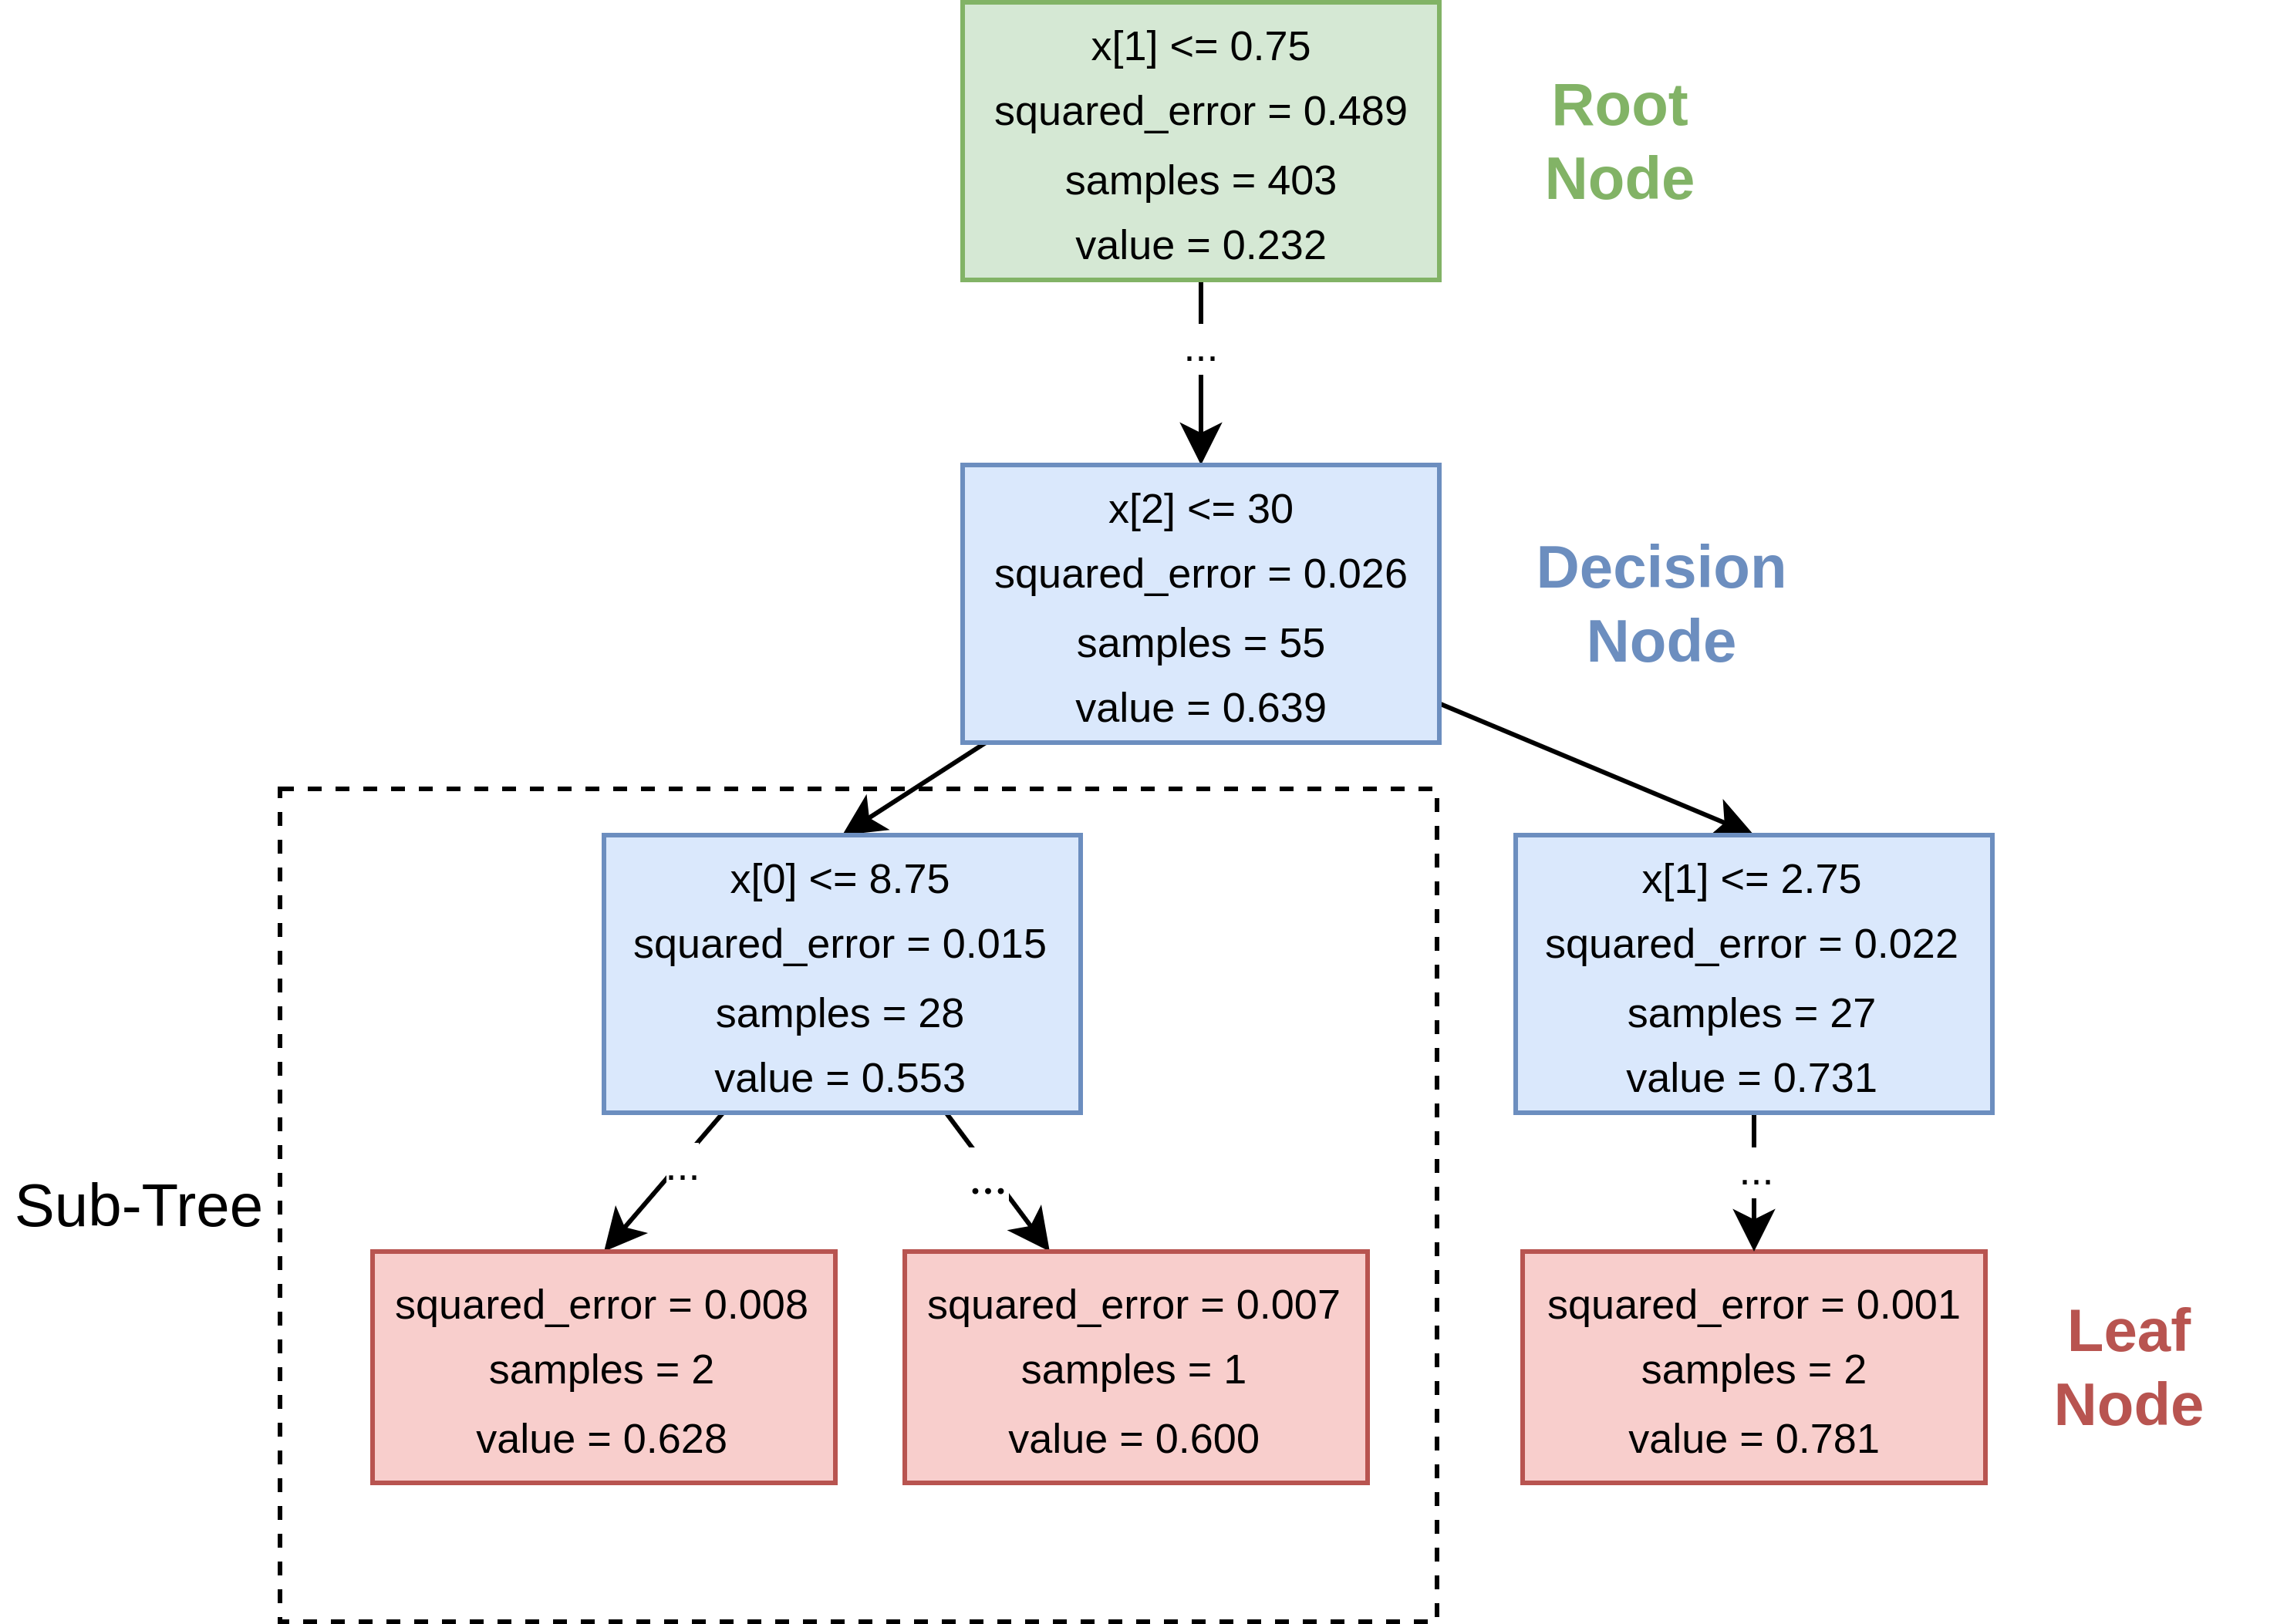
\includegraphics[width=0.7\textwidth]{chap4/images/decision_tree_example}
    \end{tcolorbox}
    \caption{Decision tree example made with \texttt{sklearn.tree.plot\_tree}~\cite{scikit-learn}.
    }
    \label{fig:dt-example}
\end{figure}

\subsubsection{Random Forest}\label{subsubsec:random-forests}
The primary issue with DT is their propensity to overfit, leading to poor generalization
performance and rendering them unsuitable for most use cases.
To tackle this problem, ensemble methods are often employed instead of a single
DT
~\cite[p. 83]{muller_introductionmachinelearning_2016}~\cite[p. 251]{liu_newmachinelearning_2012}.
In ensemble methods, multiple models such as decision trees are combined to form a single model.
To make new predictions, the predictions of each individual model are aggregated, for example by averaging the
predictions
~\cite[p. 222]{boehmke2019hands}.
%The RF algorithm builds trees independently in parallel, and then all of the trees' predictions are combined to make
%the final prediction.

The Random Forest (RF) algorithm~\cite[]{breiman_randomforests_2001} which combines multiple decision trees (weak
learners) to produce a more precise and stable prediction (strong learner)
~\cite[p. 24]{awad_efficientlearningmachines_2015}~\cite[pp. 340]{gareth2013introduction}.
This approach, known as the ``divide and conquer'' method, involves dividing the data into smaller randomized subsets
and constructing a randomized tree predictor for each subset
~\cite[p. 251]{liu_newmachinelearning_2012}.

The risk of overfitting is mitigated through subset and feature randomization, also known as bagging.
Bagging involves randomly selecting a subset of features or variables at each decision node in the decision
tree.
This process generates multiple, slightly varying copies of the dataset
~\cite[p. 341]{gareth2013introduction}.
Overfitting occurs when the algorithm learns individual data points instead of
the general pattern (see \cref{subsec:overfitting-and-underfitting}).
Each root node utilizes a unique subset of the data, and each leaf is split using a random set of features.
This approach ensures that no single tree is exposed to all the data, enabling the model to concentrate on general
patterns rather than being susceptible to noise
~\cite[p. 83]{muller_introductionmachinelearning_2016}.
Therefore bagging aids in diminishing the impact of individual data points or outliers that may have a
significant influence on a single decision tree.

The algorithm is visualized in \cref{fig:rf-example} the green decision nodes are the root nodes, blue decision nodes
are the decision nodes, and red nodes are the leaf nodes.
The red arrows indicate the decisions made by each decision tree for one specific sample.
Instead of a single decision tree, $N$ decision trees are built in the format described in \cref{fig:dt-example}.
The bagging was not visualized but every single decision tree is trained on a variation of the dataset for the before
described reasons.
The red arrows indicate the decisions made by each decision tree for one specific sample.
As a result, each decision tree independently arrives at one prediction which in this case would be a spring back value.
Averaging the predictions of all trees makes the final prediction~\cite[p. 9]{breiman_randomforests_2001}.

\begin{figure}[h]
    \begin{tcolorbox}[arc=0pt,boxrule=0.5pt]
        \centering
        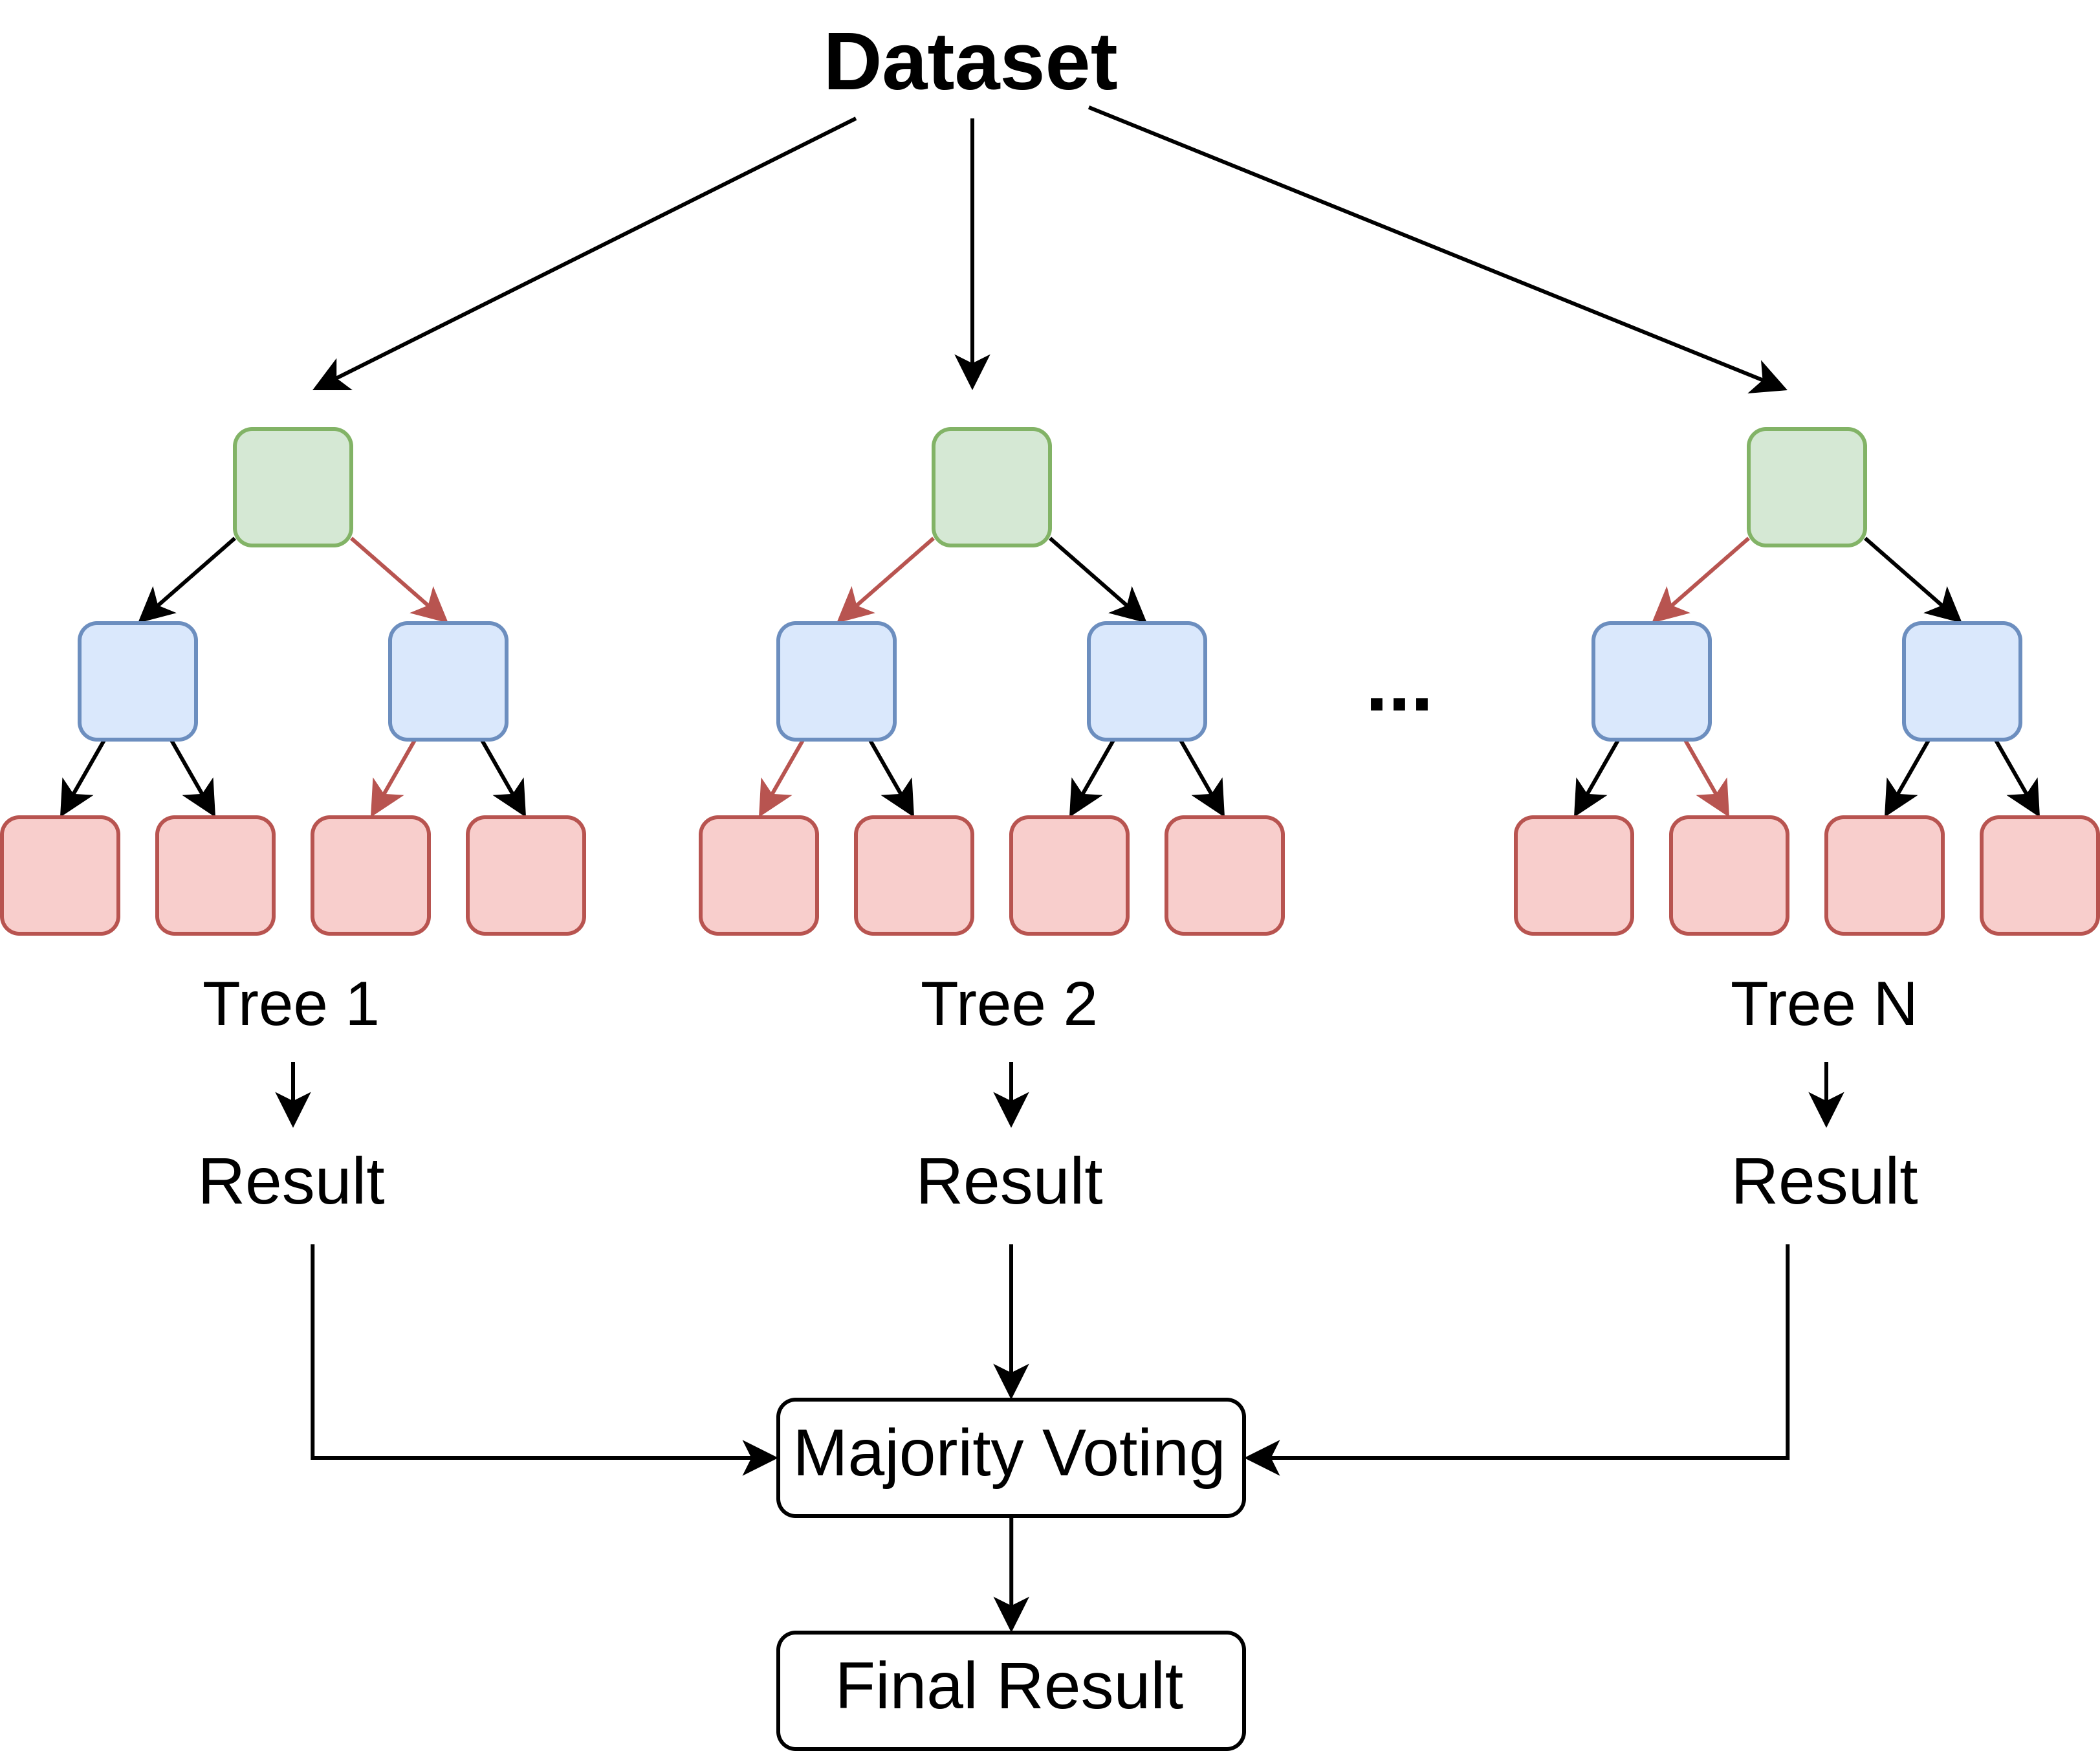
\includegraphics[width=0.6\textwidth]{chap4/images/random_forest_example}
    \end{tcolorbox}
    \caption{Visualization of the Random Forest algorithm as defined by~\cite[p.1]{breiman_randomforests_2001} (Own
    representation).
    }
    \label{fig:rf-example}
\end{figure}

The Random Forest mechanism is versatile enough to address both classification and regression problems, making it one
of the most successful
\ac{ML} methods~\cite[p. 3--4]{biau_randomforestguided_2016}~\cite[p. 25]{breiman_randomforests_2001}.

% -> Vorteile / Nachteile Random Forest
This mechanism is flexible enough to handle classifications and regression problems,this is one of the reasons that
random forests count to the most successful \ac{ML}
methods
~\cite[p. 3--4]{biau_randomforestguided_2016}~\cite[p. 25]{breiman_randomforests_2001}.


\subsubsection{Gradient Boosting Regression Tree}

A \ac{GBT} is an ensemble learning algorithm that combines multiple Decision Trees
to yield more accurate and stable predictions.
The main difference between this algorithm and the Random Forest algorithm is that the trees are trained sequentially
rather than simultaneously, with each tree correcting the errors of the previous tree.
~\cite[p. 88--89]{muller_introductionmachinelearning_2016}.
This is done with training each new tree with the residual errors of the previous tree, which is the
difference between the predicted value and can also be called the loss.
One example for a metric that can be used as loss is the Mean Squared Error (MSE) (more details in
section~\ref{subsec:correctness}).
To train a tree on the residual errors, the process is similar to train a decision tree on any other regression
task.
Instead of using the original target variable (spring back) as the label for the training data instead the
residual errors are used.
This process sequentially boost the performance of the mode with new tree added to the
ensemble, hence the name Gradient~\textit{Boosting}
~\cite[p. 222]{boehmke2019hands}

GBMs form an ensemble of shallow trees built sequentially, whereas Random Forests (discussed in
\cref{subsubsec:random-forests}) create an ensemble of independent trees with a deep structure.
Every tree in the group learns from and enhances the previous tree
~\cite[p. 221]{boehmke2019hands}.
The shallow trees are achieved through a process called pre-pruning, which means that the growth of a tree is halted
at a specific depth.
This provides the advantage of a smaller model that consumes less memory and facilitates faster prediction.
Generally, generating more trees enhances the overall performance of the
model
~\cite[pp. 74, 88--89]{muller_introductionmachinelearning_2016}.

Furthermore, the algorithm performs well without scaling the dataset and can handle a combination of binary and
continuous features
~\cite[p. 91]{muller_introductionmachinelearning_2016}

In \cref{fig:gbr-example}, we illustrate the Gradient Boosted Regression Trees (GBRT) algorithm using a sample
dataset.
The first tree is trained on the original dataset with the target variable being the spring back.
After the construction of the initial decision tree, each sample in the dataset will have a predicted value which is
likely
different from the actual spring back.
For each sample, the residual, which is the difference between the predicted and actual spring back values, is
computed.
The second tree in the sequence is then trained using these residuals as the target variable instead of the
actual spring back values.
The GBRT algorithm continues to build trees sequentially, with each tree focusing on the residuals of the preceding
tree as its target variable.
his process continues until a predefined stopping criterion is satisfied.
Such criteria may include a maximum number of trees or a threshold for minimal improvement in the final
outcome
~\cite[p. 227]{boehmke2019hands}.

\begin{figure}[h]
    \begin{tcolorbox}[arc=0pt,boxrule=0.5pt]
        \centering
        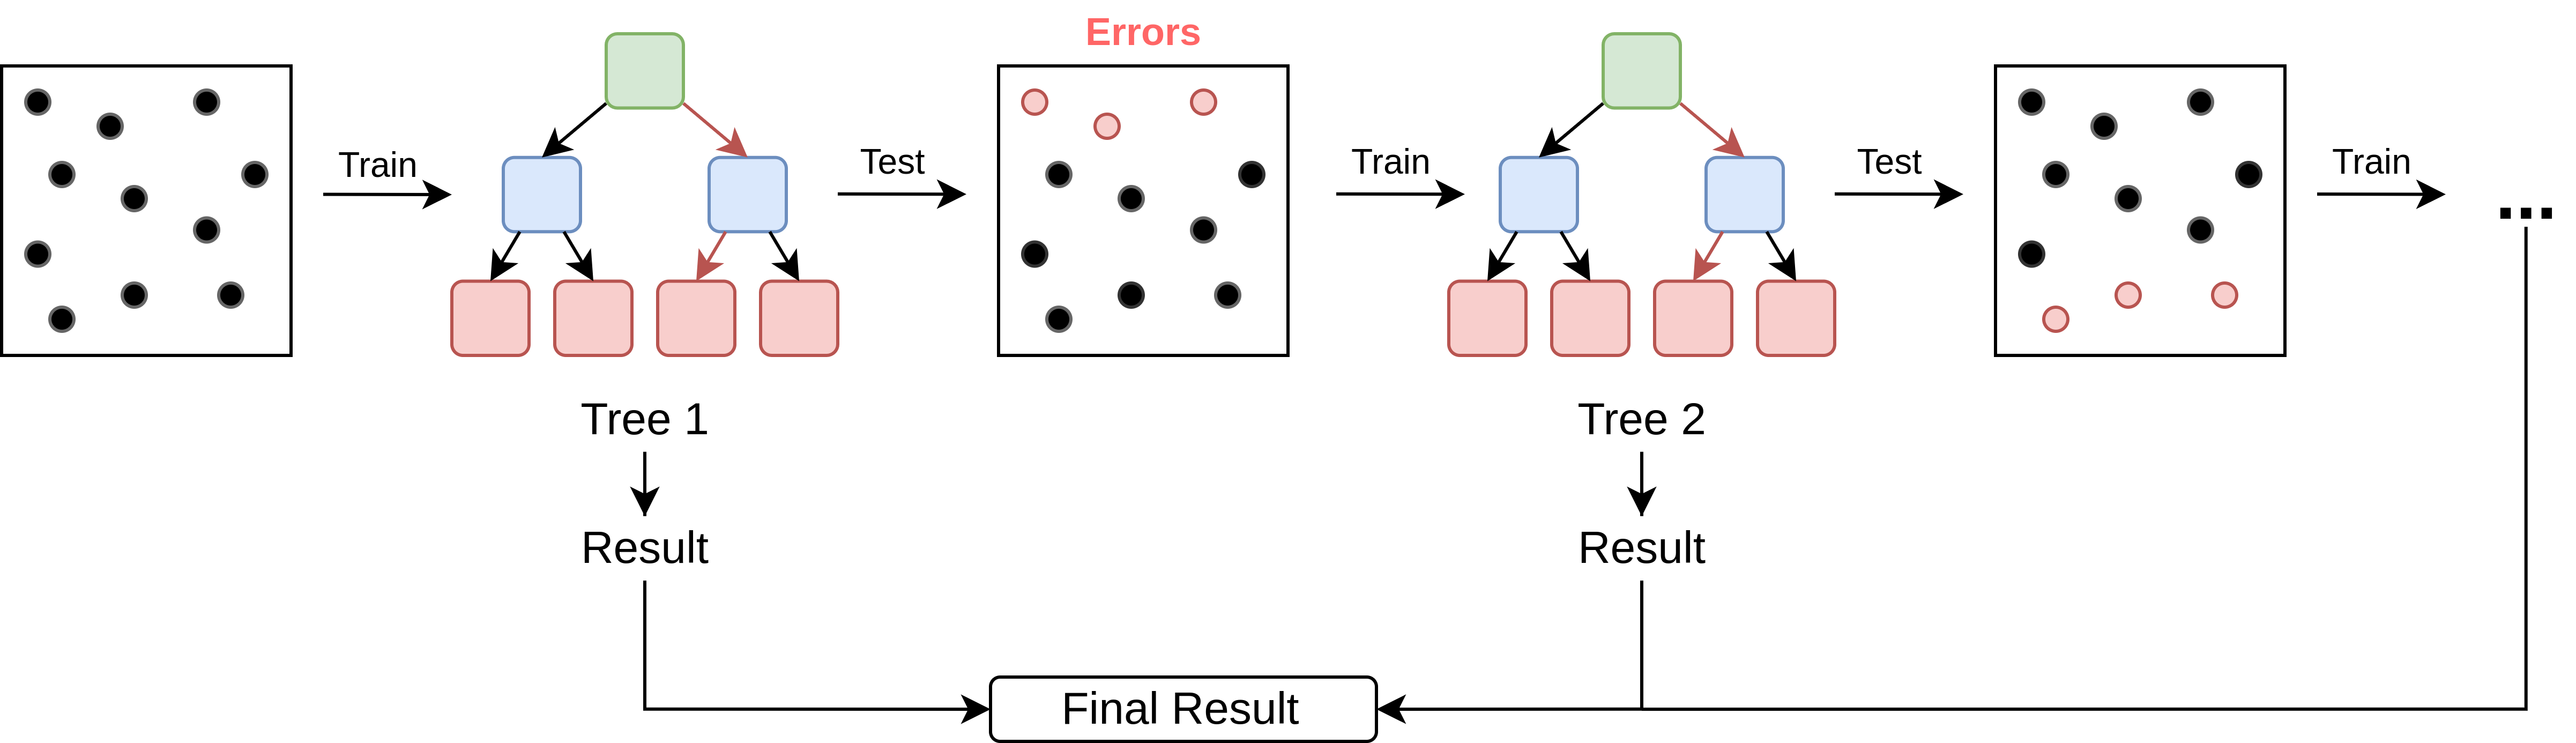
\includegraphics[width=1\textwidth]{chap4/images/gradient_boosting_example}
    \end{tcolorbox}
    \caption{Visualization of the \ac{GBR} algorithm adapted from~\cite[p. 222]{boehmke2019hands}}
    \label{fig:gbr-example}
\end{figure}



\subsubsection{Extra Trees}\label{subsubsec:extra-trees}
In the construction of a random forest, decision trees are developed using a randomly selected subset of features for
each node (see Section~\ref{subsubsec:random-forests}). To further enhance the randomness of the trees, random
thresholds can be employed for decision rules in addition to the random selection of
features~\cite[p. 351]{geron2022hands}.

An ensemble consisting of such highly arbitrary trees is referred to as an Extra-Trees (or Extremely Randomized Trees
) ensemble.
This approach generates more diverse and less correlated trees, leading to reduced variance and increased
bias
~\cite[p. 351]{geron2022hands}.
Furthermore, using ET classifiers speeds up the training process as compared to standard Random Forests, as
establishing the correct threshold for each feature at each node is one of the most time-consuming components of tree
growth
~\cite[p. 351]{geron2022hands}.

\subsection{Neural Networks}\label{subsec:neural-networks}
Another method for supervised learning involves the utilization of Neural Networks to
perform classification and regression tasks.

While this study does not go into detail about the usage of Artificial Neural Networks for spring back prediction
because that would be outside the scope of this paper.
Instead a simple Multi-Layer Perceptron (MLP) is used for the comparison with the other models. The goal is to
evaluate if the employment of Neural Networks can be a future research area.

The perceptron is inspired by the biological neuron in the brain and is the basic processing unit of a neural
network.
Each perceptron has one or more inputs from the previous perceptions or the environment and computes a weight sum of
these inputs.
The weight determines if a perceptron triggers a certain activation function and `fires' or
not.
The activation function is often a simple sigmoid function which determines a threshold for the perceptron to activate
~\cite[pp. 271--273]{alpaydin2020introduction}.

The MLP is a feedforward neural network which means that is organized into layers, with information
moving in one direction from the input layer through the hidden layers to the output
layer.
These layers are the input layer, one or more hidden layers and an output
layer
~\cite[pp. 279--280]{bishop1995neural}.
The input layer is the network's first layer and is in charge of receiving input data.
It contains the same number of nodes as the number of features in the dataset
~\cite[p. 105]{muller_introductionmachinelearning_2016}.
In this example, the neural network's input layer would be made up of three perceptrons, each of which corresponded
to one of the independent features, namely thickness, die opening, and punch penetration.
The input layer does not perform any computation and only passes the input data to the next layer, which is
\cref{fig:mlp-example} is a hidden layer.

In a fully connected neural network like the MLP each neuron in the input layer is connected to each neuron in the
first hidden layer.
While doing this each neuron multiplies the input values with the weight value associated with the connections
denoted as $w_i$
The output layer of the neural network does produce the final output of the network.
The output is calculated based on the weighted output produces by the last hidden layer
~\cite[p. 106]{muller_introductionmachinelearning_2016}.

Setting the weights to a specific values is the task of the training process and is the actual `learning' part of the
MLP.
During the training the algorithm adjusts the weights of the connections between the neurons in order to minimize
the error between the predicted and actual output.
A backpropagation algorithm is typically used to train \ac{MLP} models, by
propagating errors backwards from the output layer to the input layer in order to adjust
the weights
~\cite[p. 454]{taud2018multilayer}.

This is done in multiple steps, \cite{nielsen_neuralnetworksdeep_2015} make and example with a network to recognize
handwritten digits, this example is simplified and applied on the MLP model used in this study
(\cite[p. 12--24]{nielsen_neuralnetworksdeep_2015}):

\begin{enumerate}
    \item The input data is passed through the network, layer by layer, until it reaches the output layer and a
    result is calculated.
    This process is known as the forward pass.
    \item The error is then calculated by comparing the predicted output with the actual output.
    For example, if the projected spring back is 0.5 and the actual spring back is 0.6, the difference between these
    values is the error which can also be negative.
    \item The error is propagated backwards through the network, from the output layer to the input layer, to
    calculate the gradient of the error with respect to the network's weights and biases. To reduce the error,
    the weights are then updated in the direction of the negative gradient using an optimization algorithm such
    as gradient descent.
    \item This process is repeated iteratively for all
    samples in the training set, updating the weights and bias steps after each batch, until the error function
    reaches a minimum value or a stopping criterion is met.
\end{enumerate}

In summary, backpropagation is a process that uses the error between the predicted and actual output to update the
weights and biases of a neural network.
By iteratively updating the weights and biases, the network can learn to make more accurate predictions
~\cite[p. 53--57]{nielsen_neuralnetworksdeep_2015}.

Usually a weight $x_0$ is included in the perceptron model as an intercept value to increase its generality.
It is typically represented as the weight coming from an additional bias unti that always has a value of +1.
\cref{fig:mlp-example} show a simplified visual representation of an MLP used in this study.
It uses the tree input $V$, $t$, $y_p$ from the used dataset, the perceptrons in the input layer are denoted as $x_i$,
the perceptrons in the hidden layer as $a_i$ and the perceptron in the output layer as $f(X)$.
The weights of the connections between the perceptrons are denoted as $w_i$.

\begin{figure}[h]
    \begin{tcolorbox}[arc=0pt,boxrule=0.5pt]
        \centering
        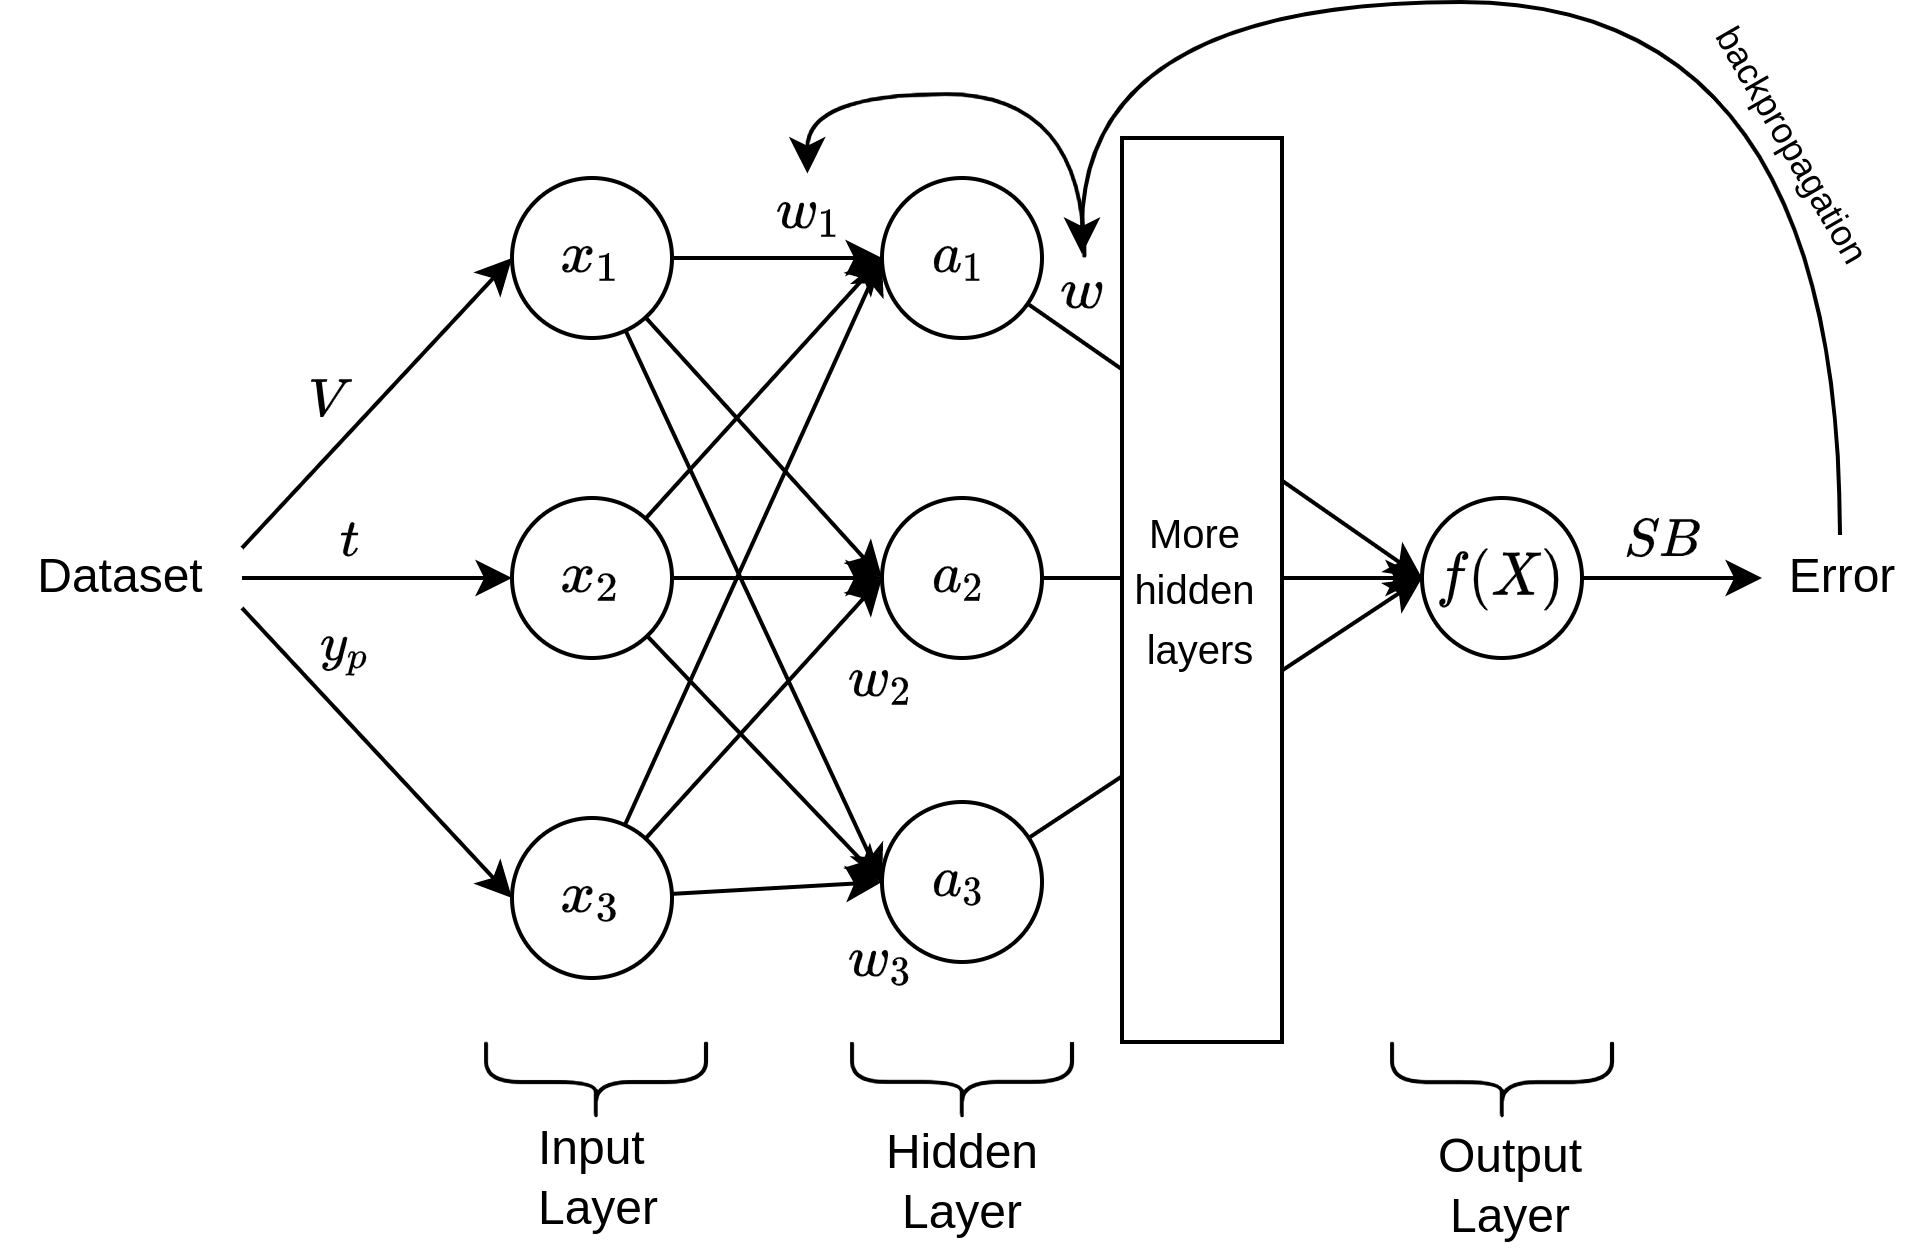
\includegraphics[width=0.8\textwidth]{chap4/images/mlp_example}
    \end{tcolorbox}
    \caption{Visual representation of a Multi-layer Perceptron. Modeled after decription of
    \cite{nielsen_neuralnetworksdeep_2015} and applied on the scenario of this study
        (own repsentation). }
    \label{fig:mlp-example}
\end{figure}


\section{Model Training}\label{sec:model-training}
Supervised learning involves training machine learning algorithms a dataset which contains the inputs features as well
as target feature in this study spring back.
In order to evaluate how well the model generalizes to new, unseen data, it is necessary to
split the dataset into training and testing sets.
This involves taking some samples from the original dataset and using them exclusively to test the trained models.

\subsection{Training-Test Split}\label{subsec:training-test-split}
\cref{fig:train_test_split} displays the dataset partitioned into training and testing sets for the models used in
this study.
Specifically, the samples with a die opening of 30 were reserved for testing, while the remaining data was used for
training.
While a random train-test split can often yield better model performance, but this may not evaluate the model's ability
to predict new data with a different die opening.

The decision to use a die opening of 30 was based on its central location within the selected dataset, allowing the
models to predict this value accurately. Furthermore, removing data from the middle of the parameter space during
training is expected to improve model performance and promote generalization to new data.
All models were trained on the same dataset.
For algorithms with hyper-parameters, Grid-Search Cross-validation was used to set the them accordingly.
The full hyper-parameters for each model are listed in \href{sec:hyper-parameters}.

\subsection{Setting the Hyper-Parameters}\label{subsec:hyper-parameters}
Prior to training a machine learning model, users of machine learning implementations like the ons found in
\texttt{sci-kit learn} generally need to manually choose a Machine Learning algorithm and configure one or more model
parameters, known as hyper-parameters~\cite[pp. 1]{claesen2015hyperparameter}.
The chosen hyper-paramters significantly influence the performance of the resulting model and difference a lot from use
case to use case~\cite[pp. 1]{claesen2015hyperparameter}.
As a result, it is critical to set the proper parameters.

A few examples of hyper-parameters for a Random-Gorest modelcitescikit-learn include the number of trees, the number
of features to consider when looking for the best split, and the maximum depth of the tree
~\cite{scikit-learn}.
The use of a grid-search cross-validation is a popular method to discover the best hyper-parameters.
This is the approach used in this study and was described in \cref{subsubsec:grid-search} `Grid Search'.
The hyper-parameters utilized for each model are listed in~\cref{sec:hyper-parameters} to allow the reader to
duplicate the outcomes of this study.
This data can also be seen in the study's source code.


\section{Result of the Build-Phase}\label{sec:results-build-phase}

The design and development of the machine learning models have been completed, marking the end of the `Build' phase
in this study.
All models were implemented using the libraries listed in \cref{tab:libraries} and the source
code is publicly available on GitHub at:

\url{https://github.com/Philipp0205/Master-Thesis-Code}

Each model has its own folder under the sub-directory \texttt{learner}, containing the model and any additional files
associated with the learner.
To run the model, simply execute the \texttt{main} function.
The dataset used in \cref{sec:dataset-generation} ``Dataset Generation'' and subsequent sections can be found in
the sub-directory \textit{data/dataset}.
The dataset is structured into different folders for each die opening used
to generate the data.
Additional files for the dataset, such as a visualization of how the spring back was calculated
for every single bend, can also be found in that folder.